\documentclass{beamer}
\usepackage{comment}
\usepackage{multirow}
\usepackage{amsmath}
\usepackage[utf8]{inputenc}
\graphicspath{ {./images/} }

%Information to be included in the title page:
\title{MicroDrift with Bayesian Covertrees}
\author{Sven Cattell}
\date{CAMLIS, 2021}

\AtBeginSection[]
{
  \begin{frame}
    \frametitle{Table of Contents}
    \tableofcontents[currentsection]
  \end{frame}
}

\begin{document}

\frame{\titlepage}
\begin{frame}
\frametitle{About Me}
\begin{itemize}
\item Ph.D. in Algebraic Topology from JHU
\item Very involved in the AI Village
\item Formerly at Endgame / Elastic
\end{itemize}
\end{frame}

\begin{frame}
\frametitle{Table of Contents}
\tableofcontents
\end{frame}

\section{Introduction}

\begin{frame}
\frametitle{Problem Formulation}
\begin{center}
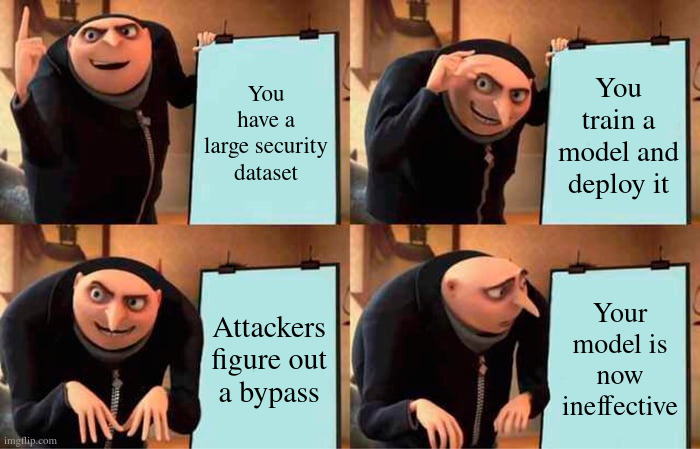
\includegraphics[scale=0.4]{grue_meme.jpg}
\end{center}
\end{frame}

\begin{frame}
\frametitle{Previous Work: Chronological Drift}
\begin{center}
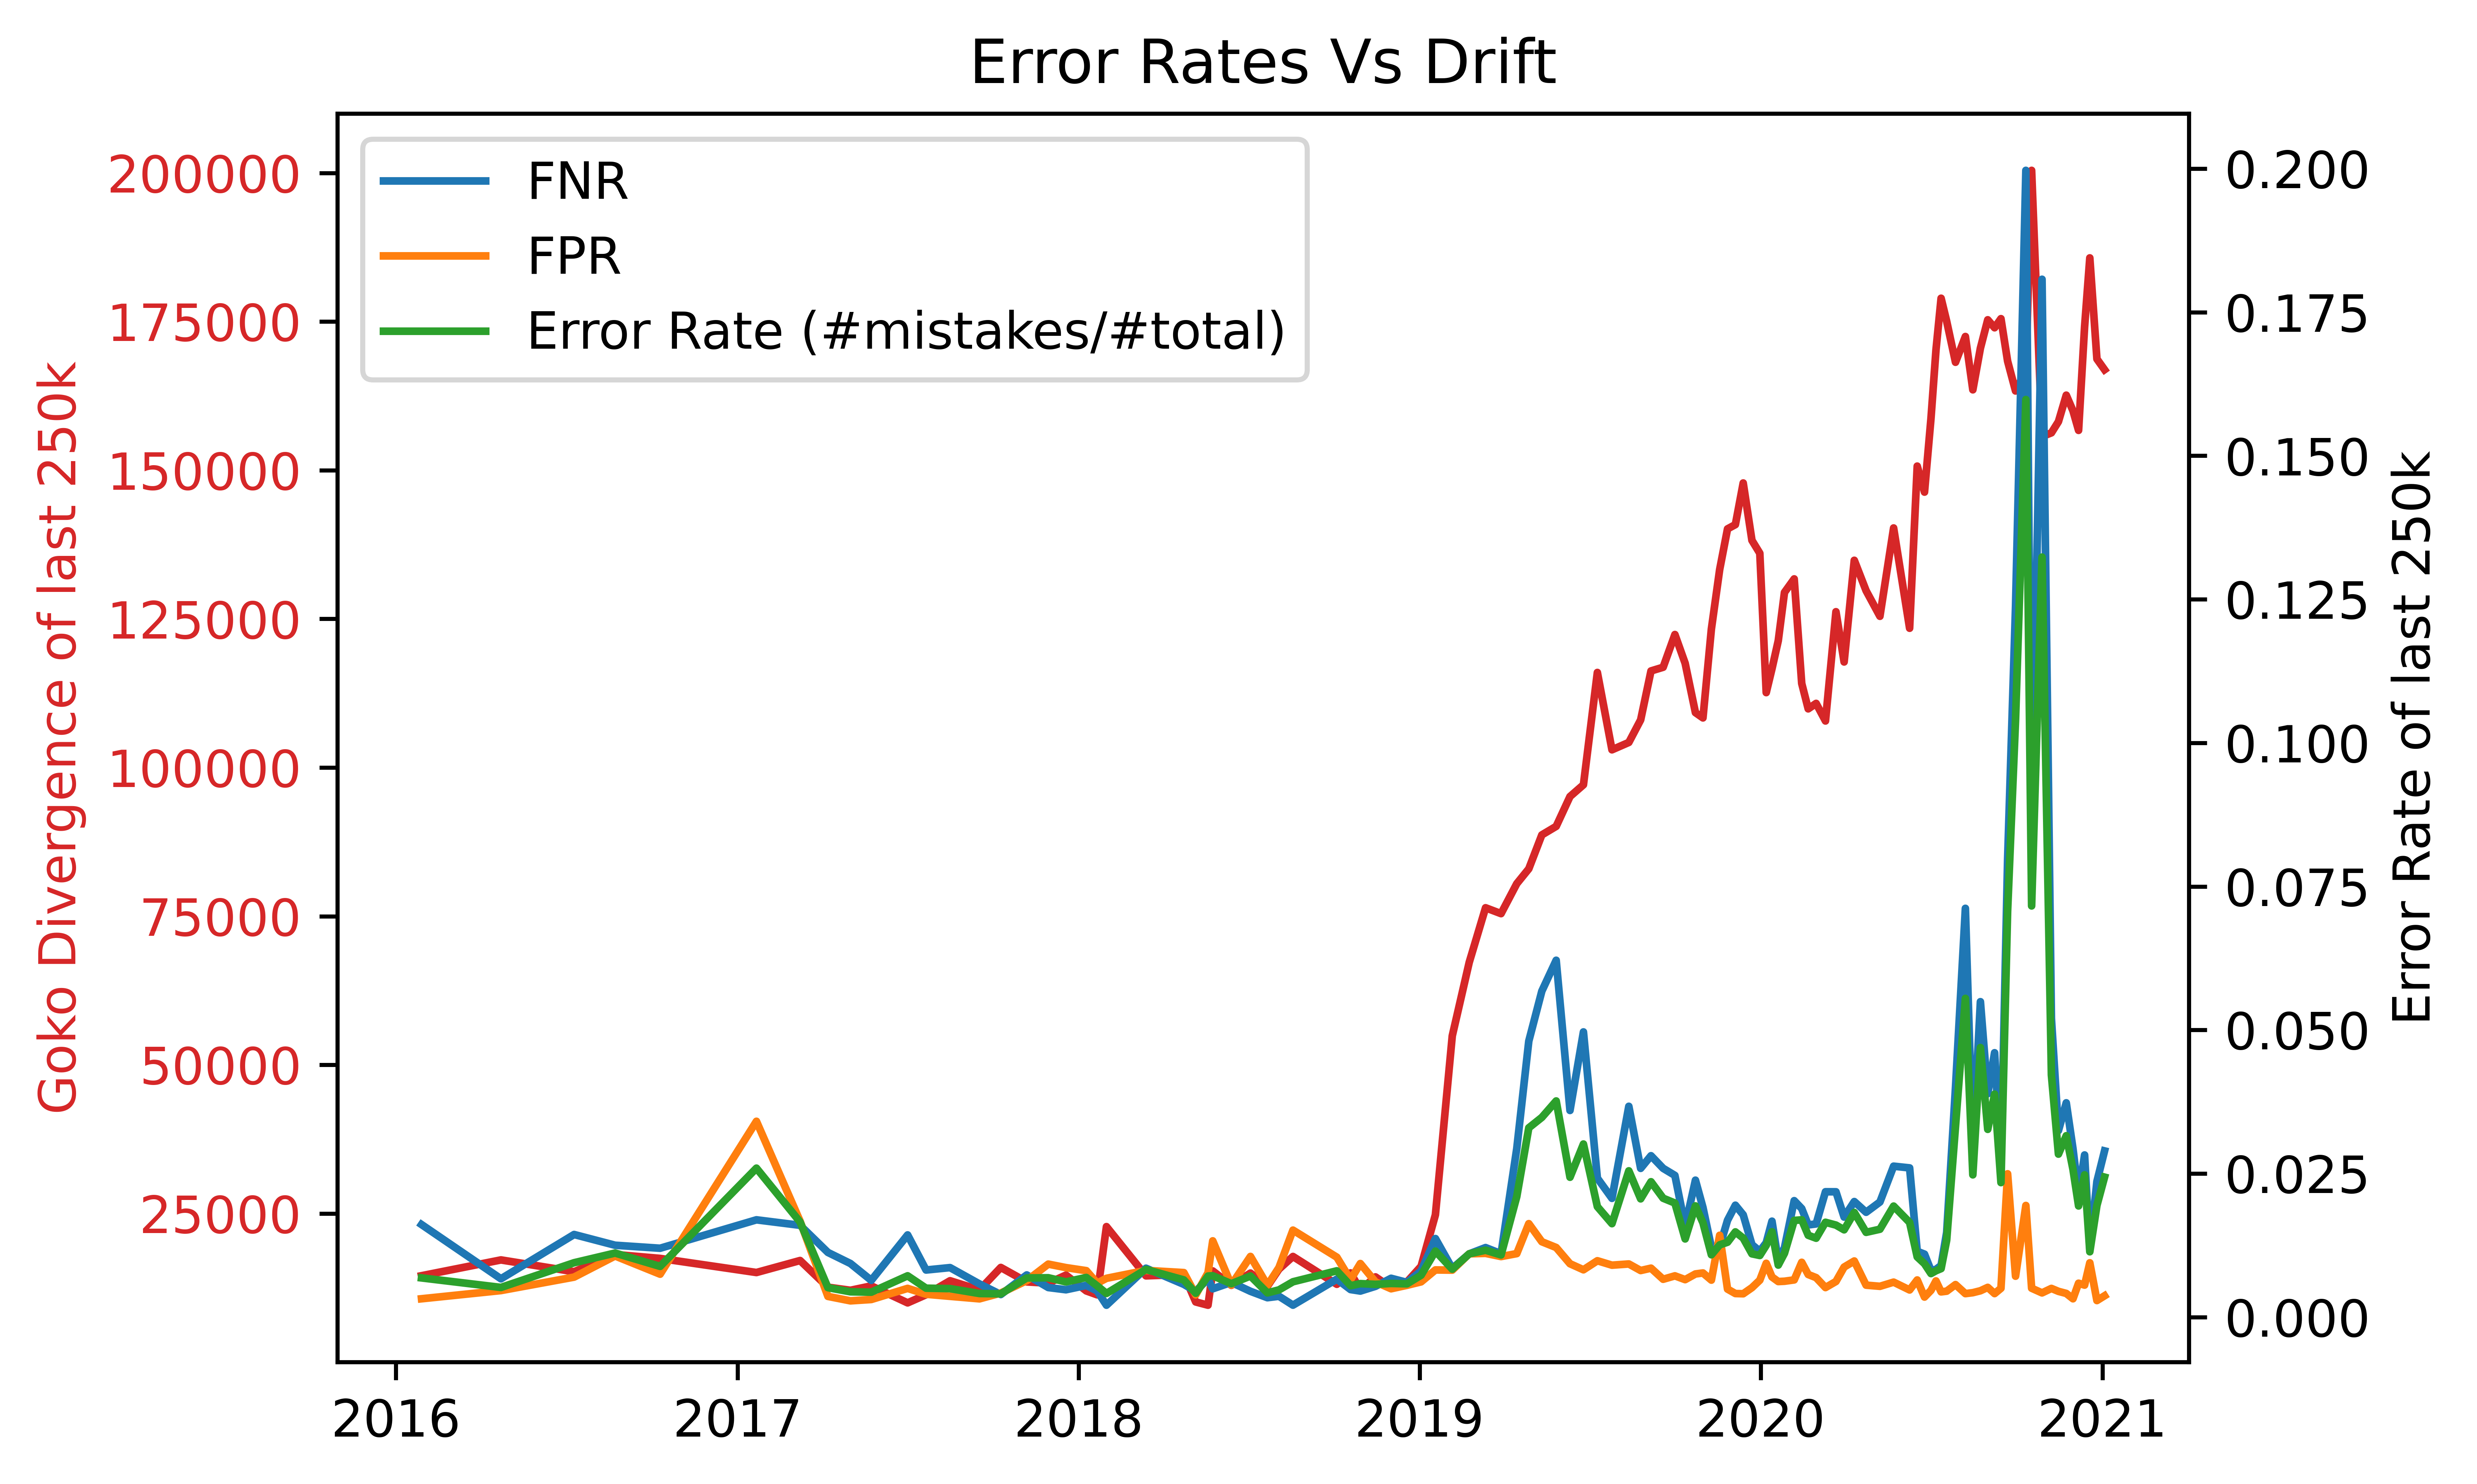
\includegraphics[scale=0.6]{overall_vs_error.png}
\end{center}
Work done at Elastic, published at ICLR
\end{frame}

\begin{frame}
\frametitle{Problems With Previous Work}
\begin{itemize}
\item Doesn't model the efficacy metrics well
\item Not that actionable, just "Retrain when KL-Div exceeds X" 
\item There's way more detail than just a single metric in the method
\end{itemize}
\end{frame}

\begin{frame}
\frametitle{Objective of This Talk}
\begin{center}
Tell me where there's a problem in my dataset, not just that there's a problem.

\vspace{20px}

Where am I being attacked/bypassed? 

Where is that new malware family? 

Where is that new popular spam technique?
\end{center}
\end{frame}

\begin{frame}
\frametitle{Types of Bypass}
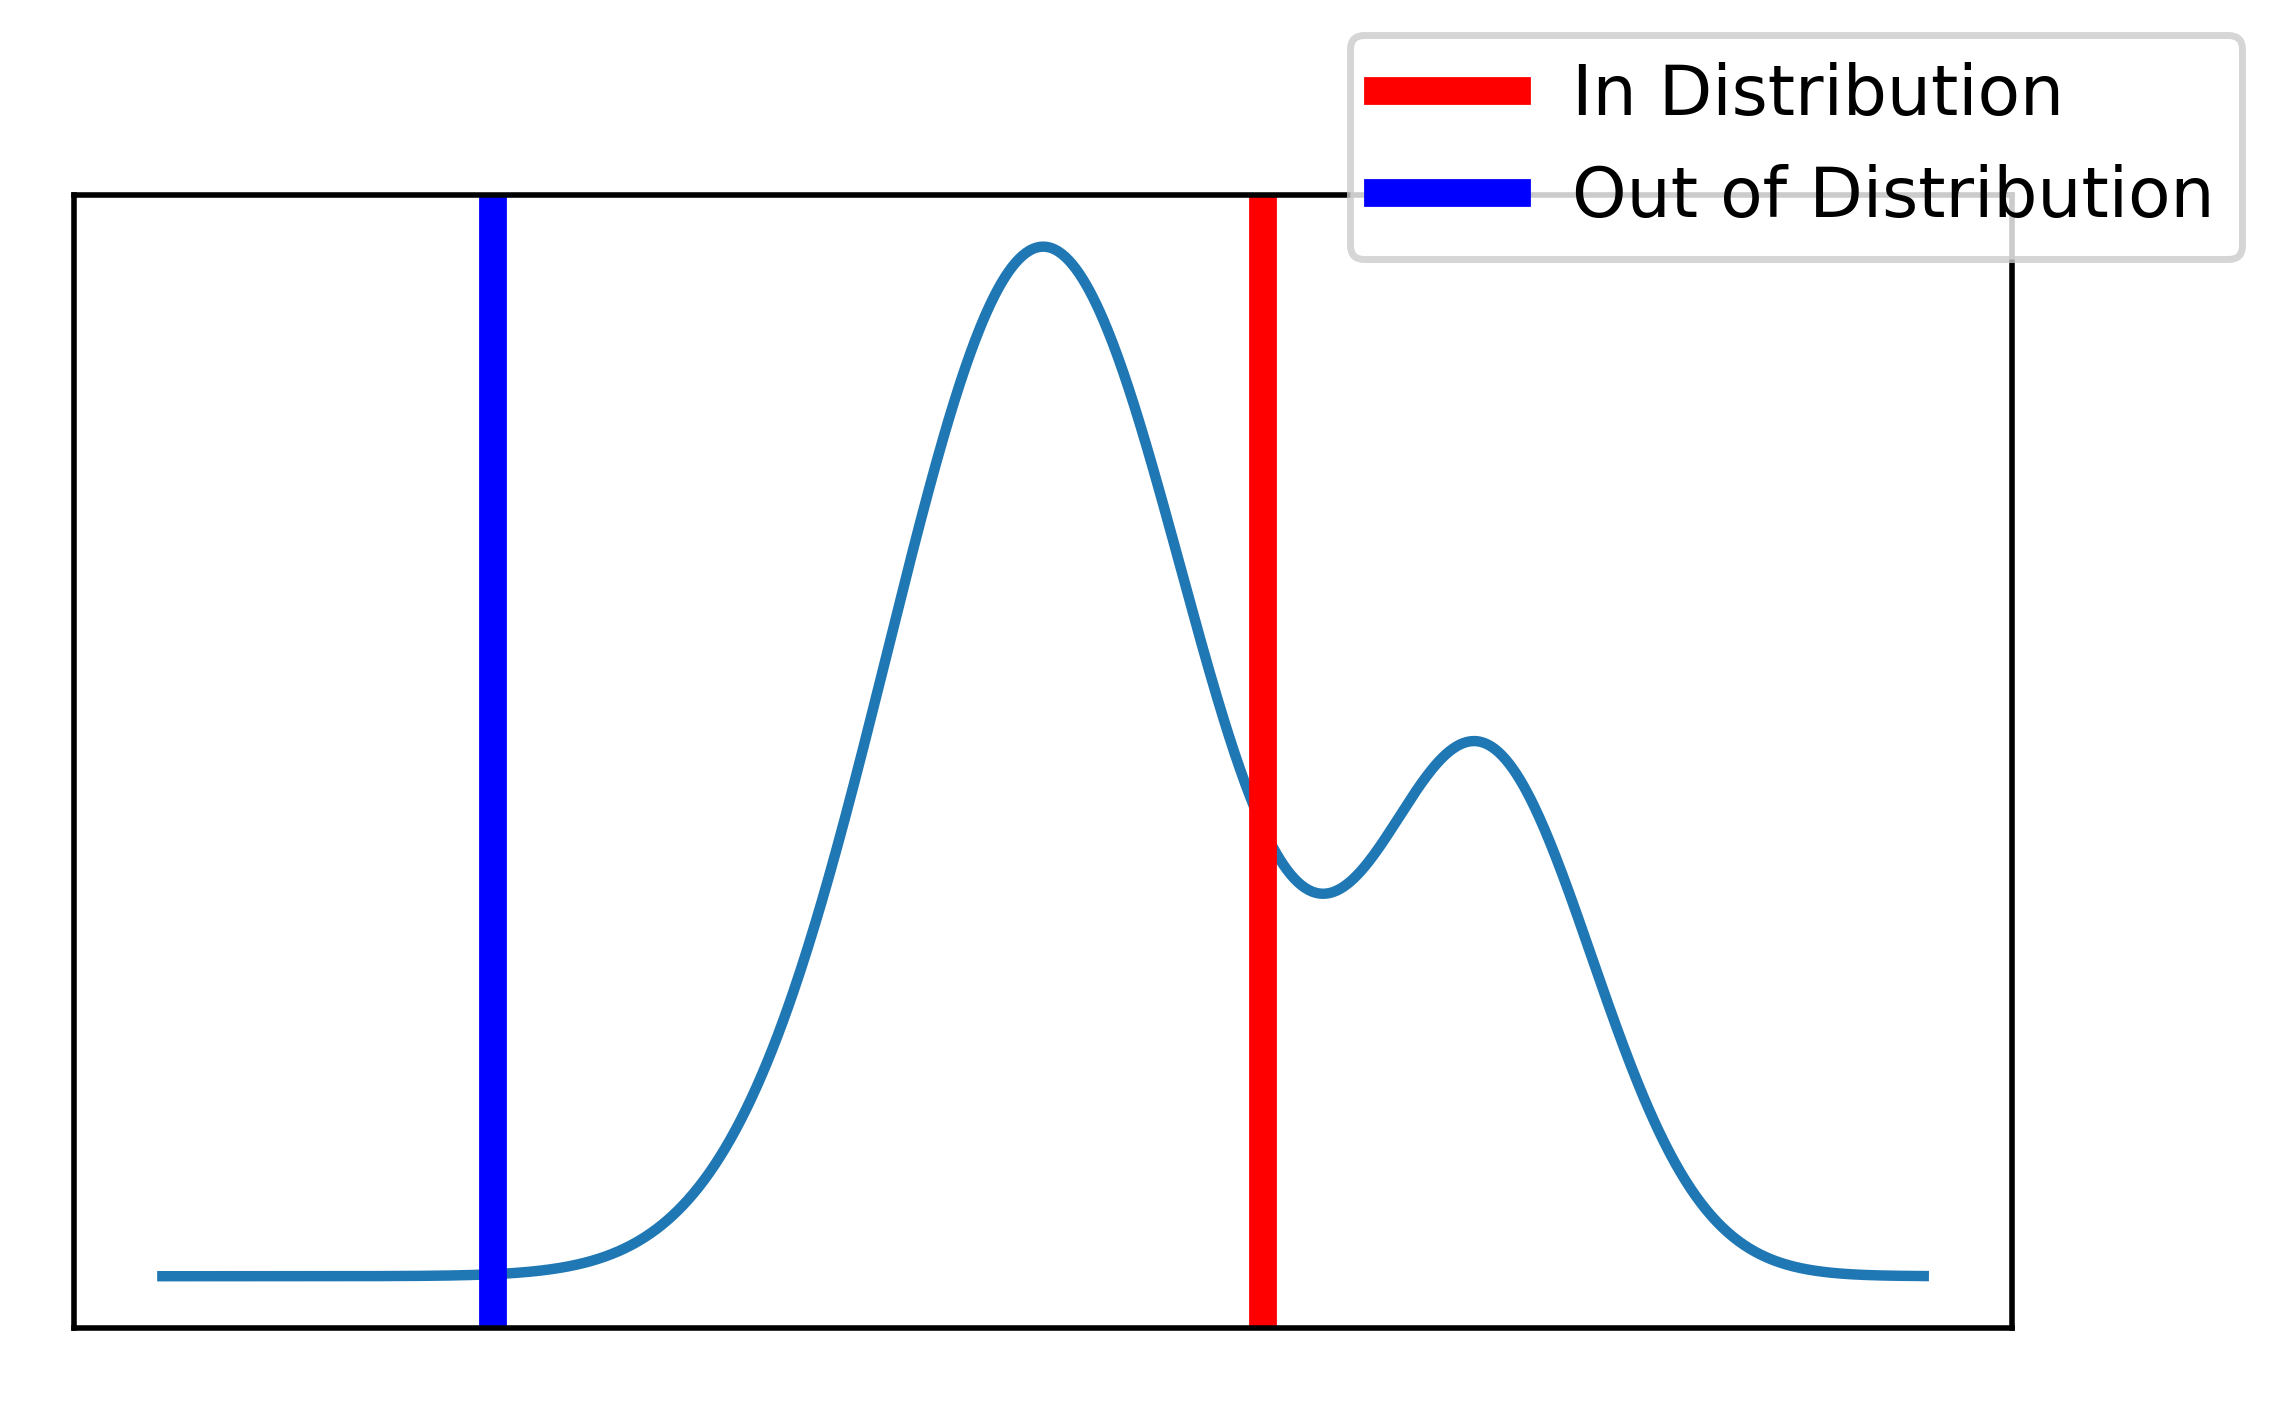
\includegraphics[scale=1]{in_vs_out.png}
\end{frame}

\begin{frame}
\frametitle{What I'm Actually Doing}
\begin{itemize}
    \item We have a dataset, and model. 
    \item Queries stream in from anonymous users.
    \item One user has an in-distribution "bypass" they are repeating.
    \begin{itemize}
        \item Building an attack with ZOO, or HopSkipJump.
        \item Spamming their spam everywhere.
    \end{itemize}
    \item The bad user's queries only account for a small percentage of total traffic.
    \item \emph{We want to isolate that user's queries as best as possible.}
\end{itemize}
\end{frame}

\section{Covertree Background}

\begin{frame}
    \frametitle{Definition}
    A \emph{covertree} over a dataset $X = \lbrace x_1, \dots x_n \rbrace$ is a filtration of a dataset into $m$-\emph{layers}, with a scale base of $S$
    $$\{x_r\} = C_k \subset C_{k-1} \subset \dots \subset C_{k-m} = X,$$
    which satisfies the following properties:
    \begin{enumerate}
        \item \emph{Covering Layer}: For each $x_j \in X$ and $i \in \{k,\dots k-m\}$, there exists $p \in C_i$ such that $d(x_i,p) < s^i$.
        \item \emph{Covering Tree}: For each $p \in C_{i-1}$ there exists $q \in C_i$ such that $d(p,q)<s^i$.
        \item \emph{Separation}: For all $p,q \in C_i$, $d(p,q) > s^i$.
    \end{enumerate}
\end{frame}

\begin{frame}
\frametitle{Lets's build one, Level 1}
\begin{center}
    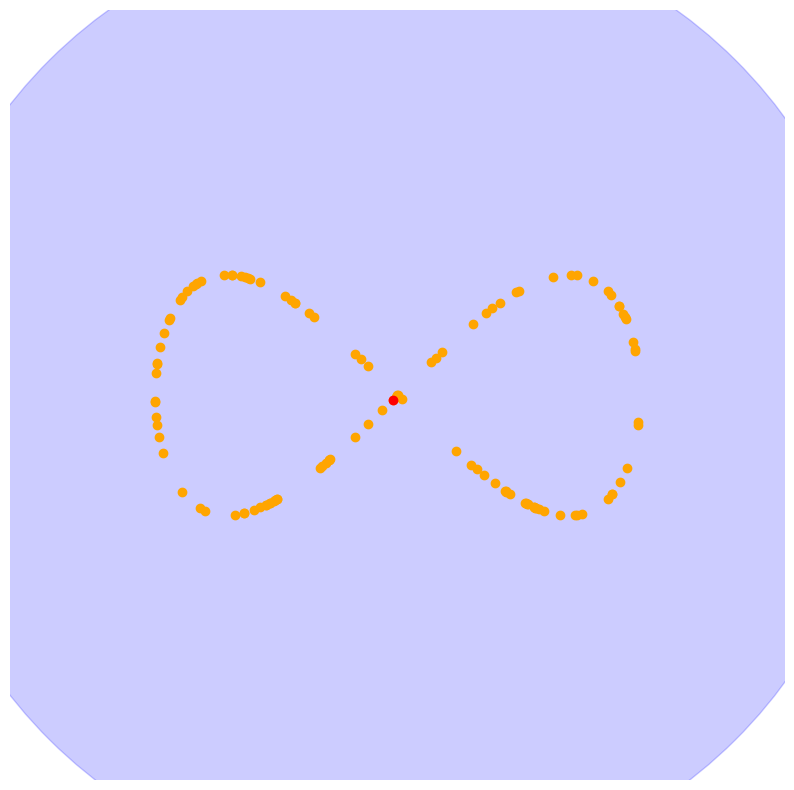
\includegraphics[scale=0.4]{2d_vis_ 1.png}
\end{center}
\end{frame}

\begin{frame}
\frametitle{Lets's build one, Level 0}
\begin{center}
    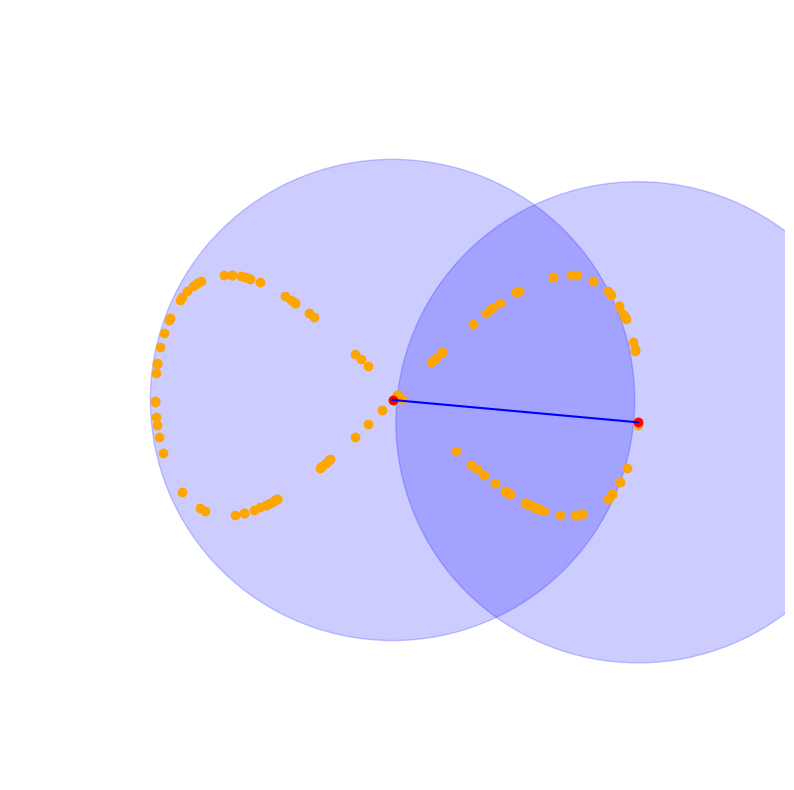
\includegraphics[scale=0.4]{2d_vis_ 0.png}
\end{center}
\end{frame}

\begin{frame}
\frametitle{Lets's build one, Level -1}
\begin{center}
    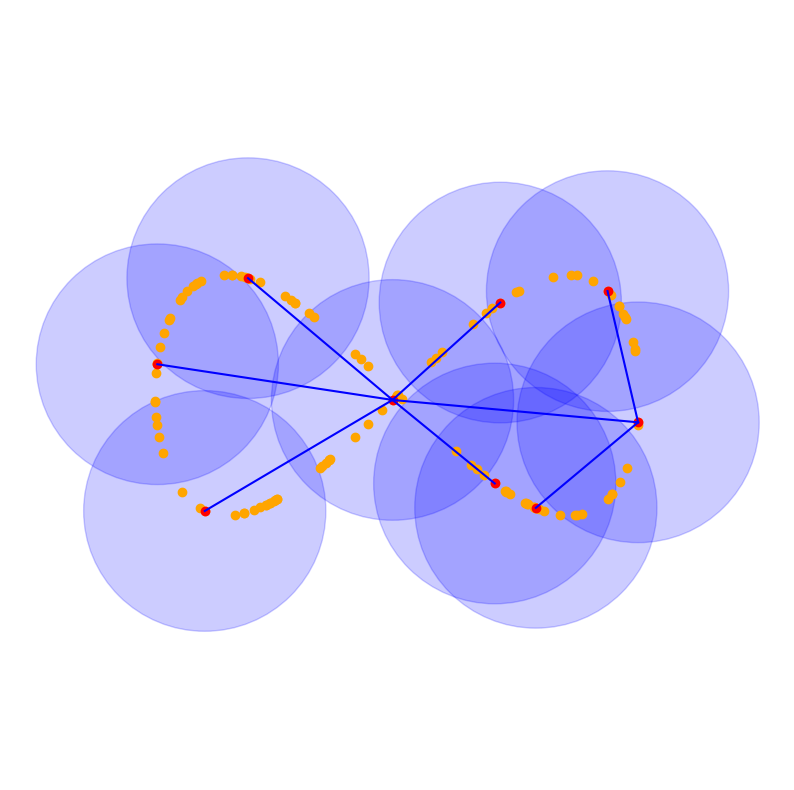
\includegraphics[scale=0.4]{2d_vis_-1.png}
\end{center}
\end{frame}

\begin{frame}
\frametitle{Lets's build one, Level -2}
\begin{center}
    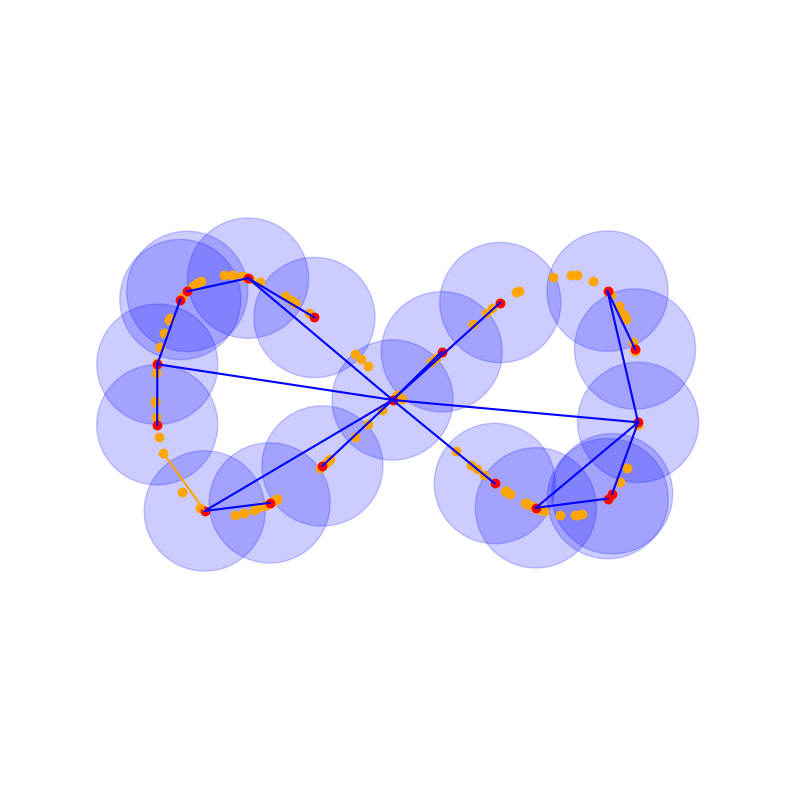
\includegraphics[scale=0.4]{2d_vis_-2.png}
\end{center}
\end{frame}

\begin{frame}
\frametitle{How A Covertree Partitions Space, Level 1}
\begin{center}
    
\includegraphics[scale=0.6]{partition_0.png}
\end{center}
\end{frame}

\begin{frame}
\frametitle{How A Covertree Partitions Space, Level 0}
\begin{center}
    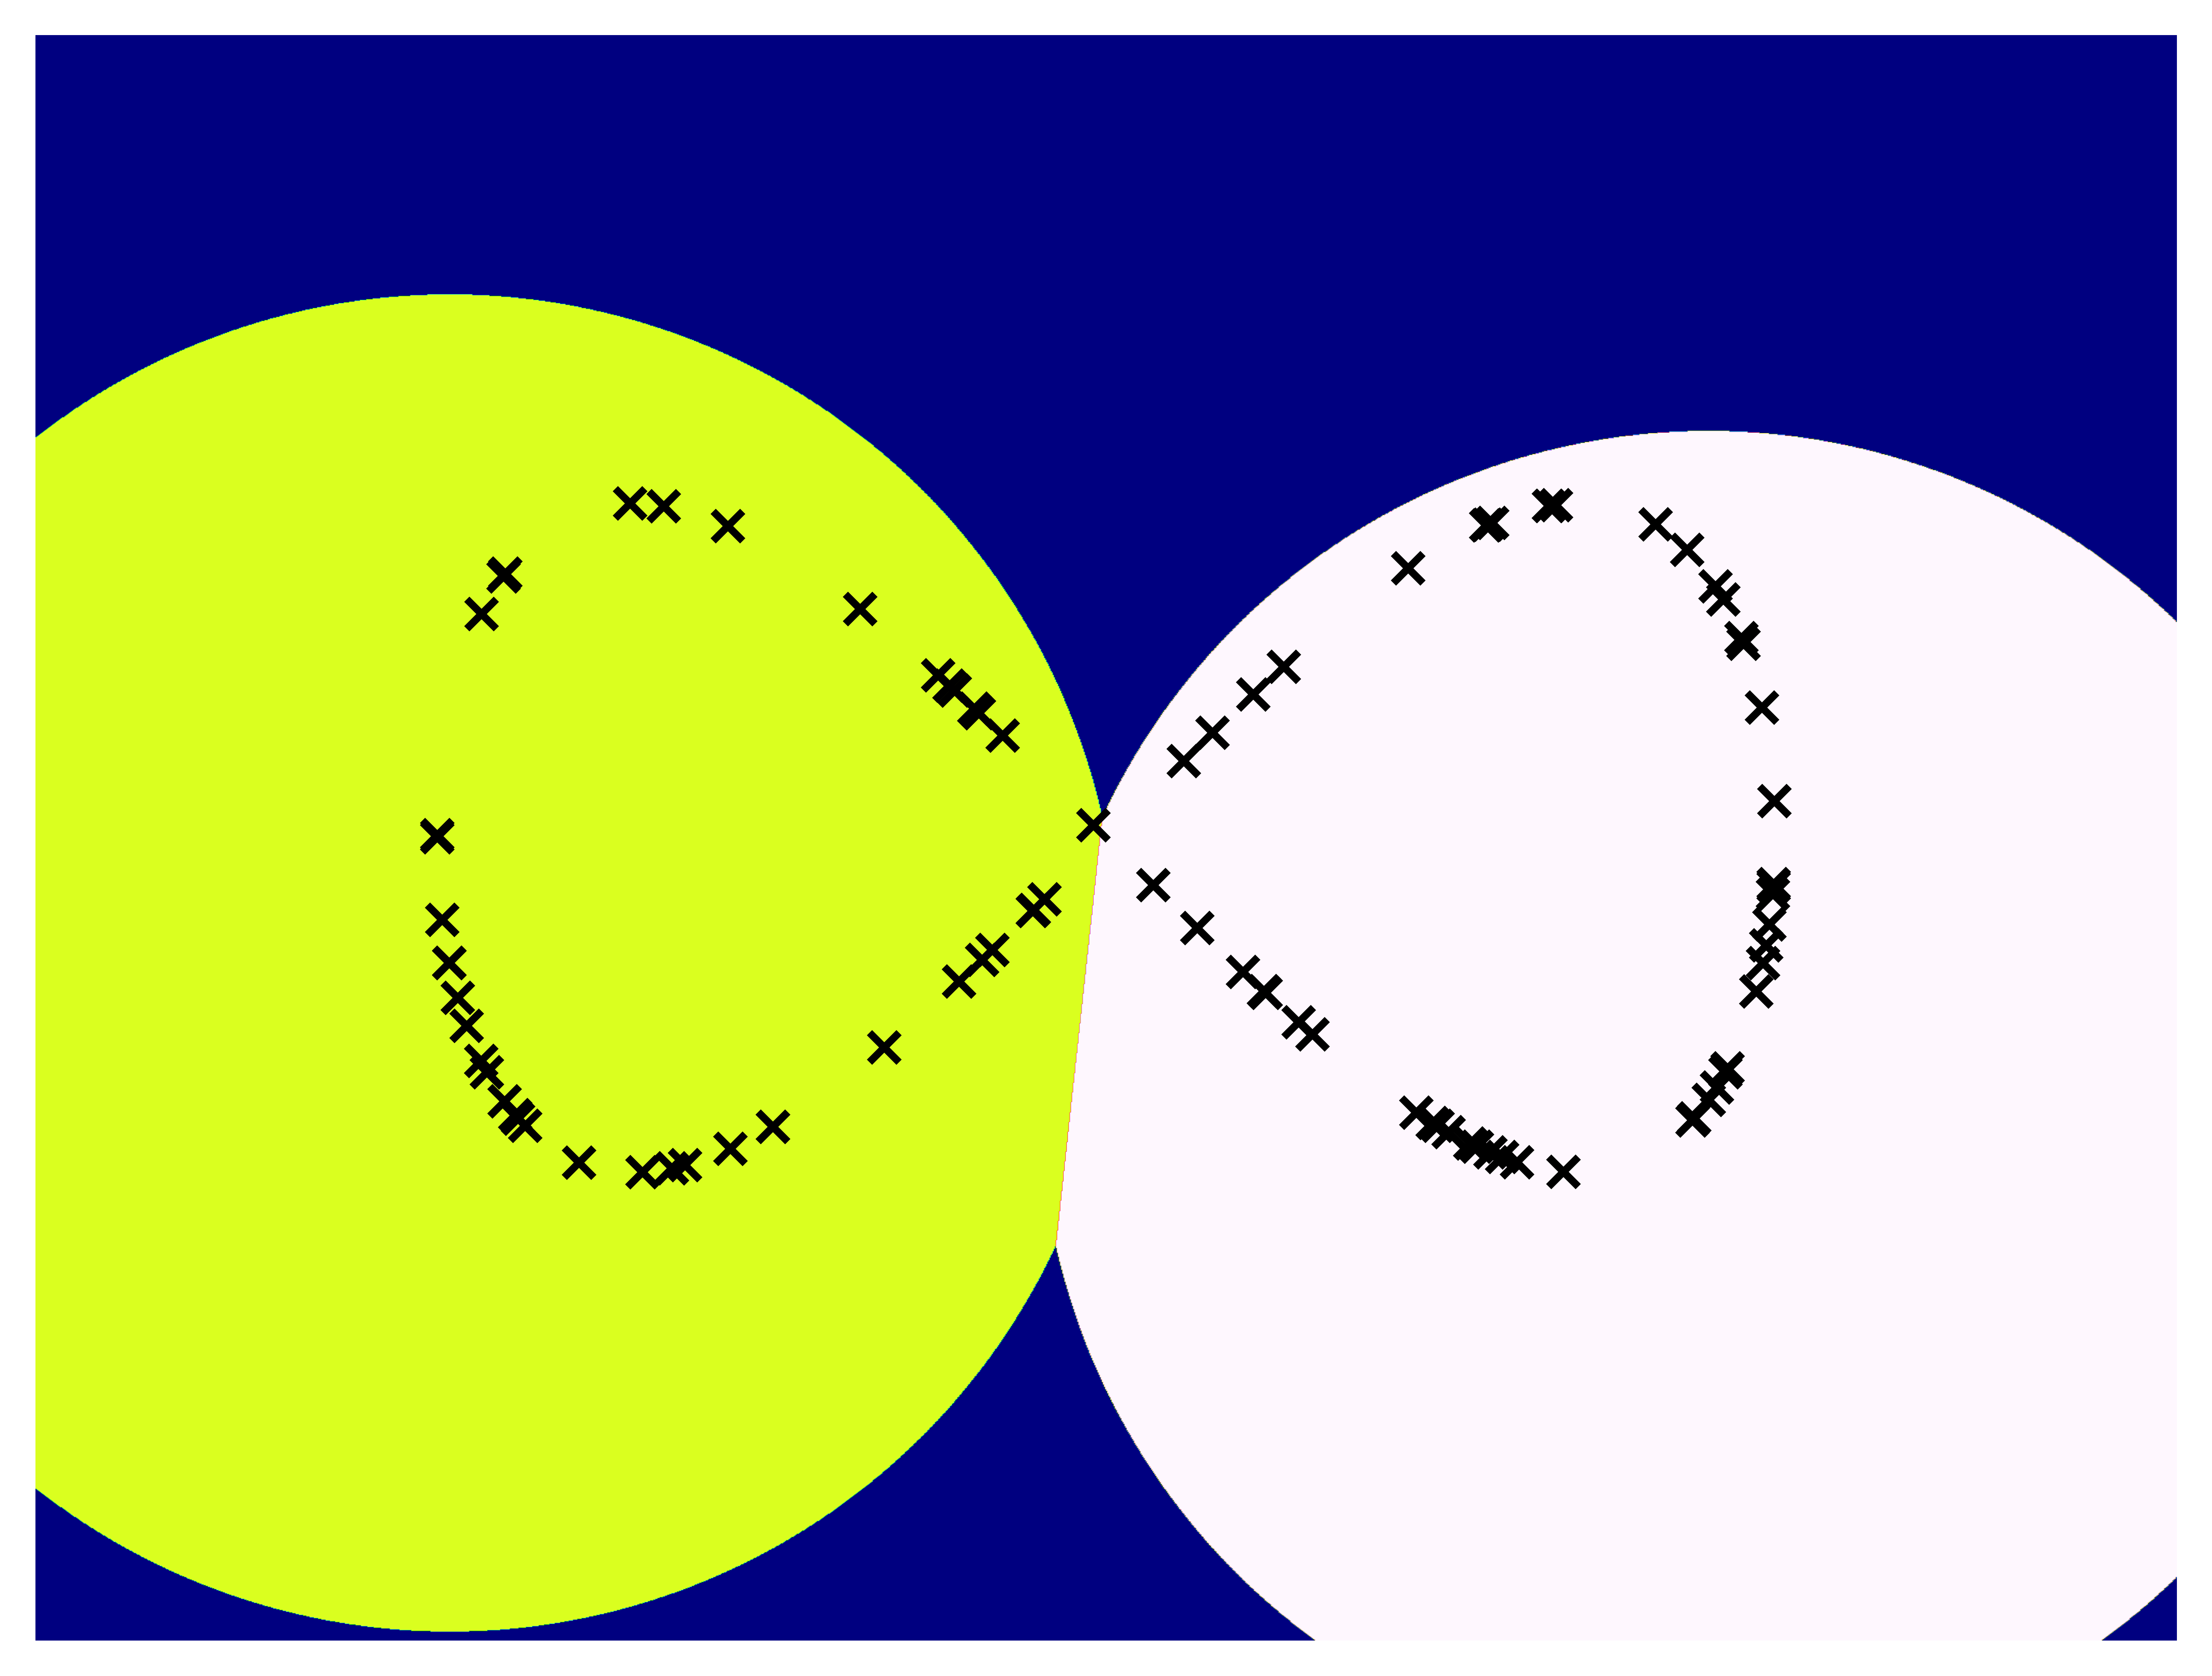
\includegraphics[scale=0.6]{partition_1.png}
\end{center}
\end{frame}

\begin{frame}
\frametitle{How A Covertree Partitions Space, Level -1}
\begin{center}
    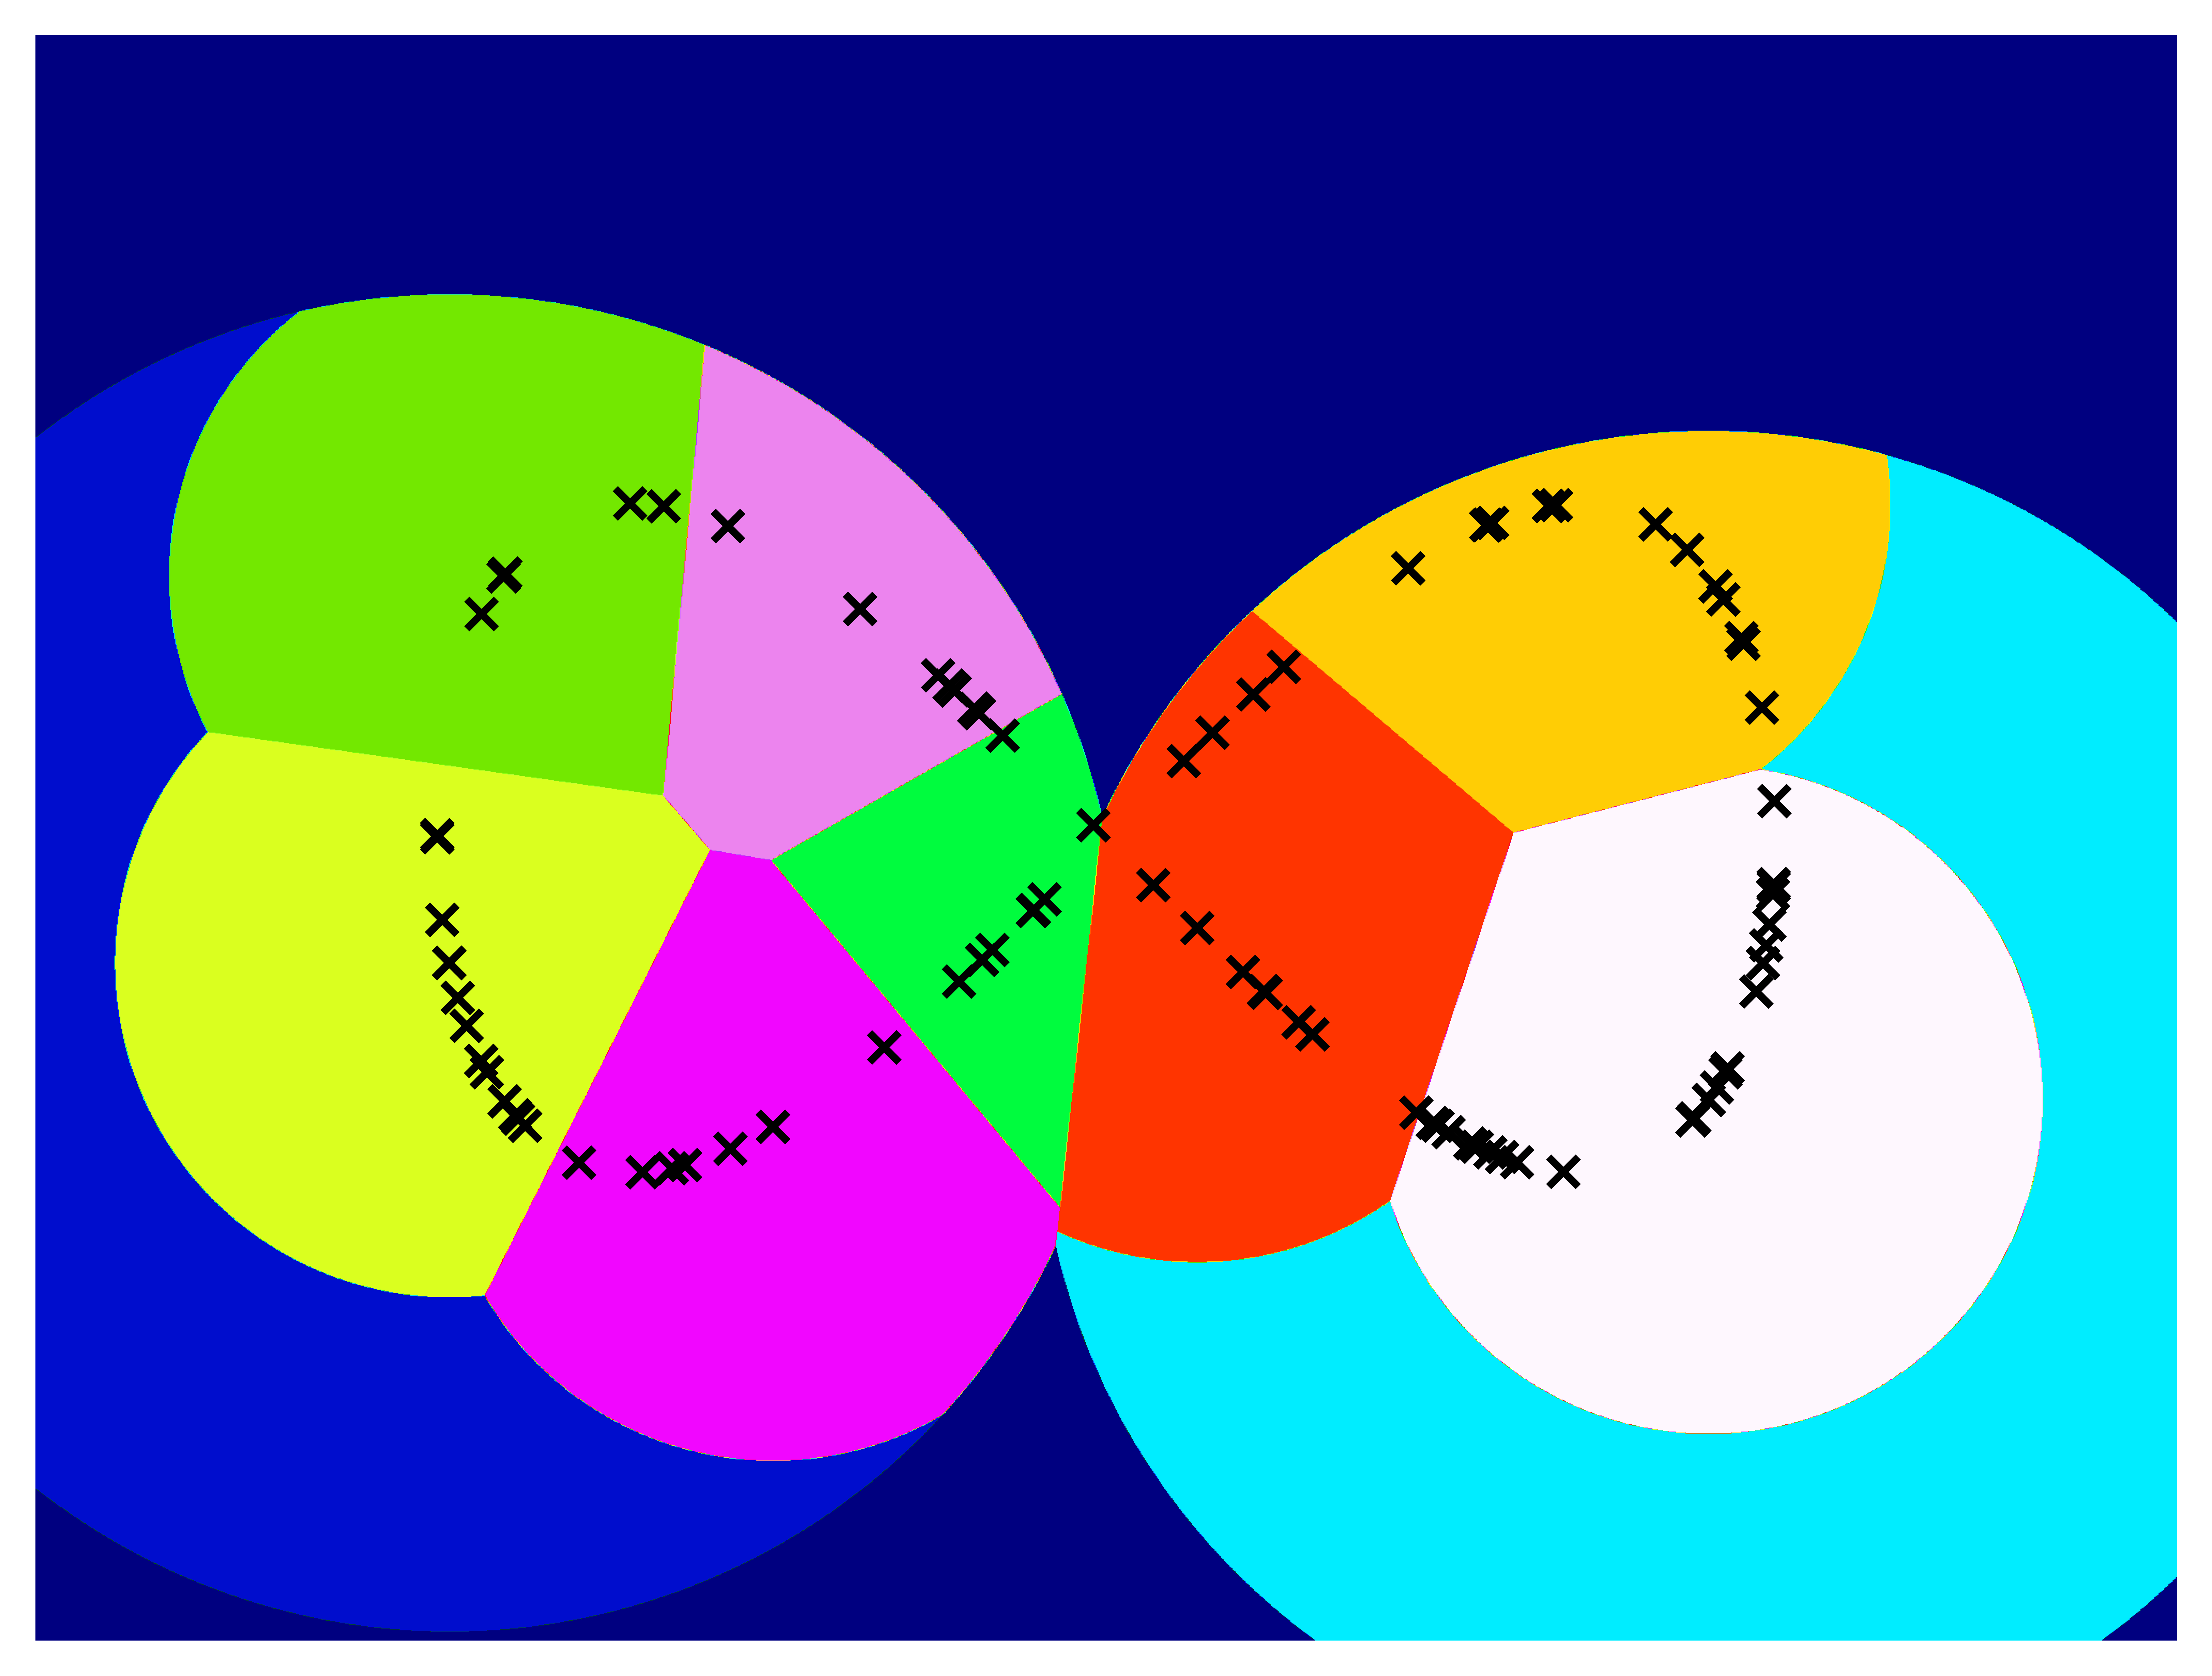
\includegraphics[scale=0.6]{partition_2.png}
\end{center}
\end{frame}

\begin{frame}
\frametitle{How A Covertree Partitions Space, Level -2}
\begin{center}
    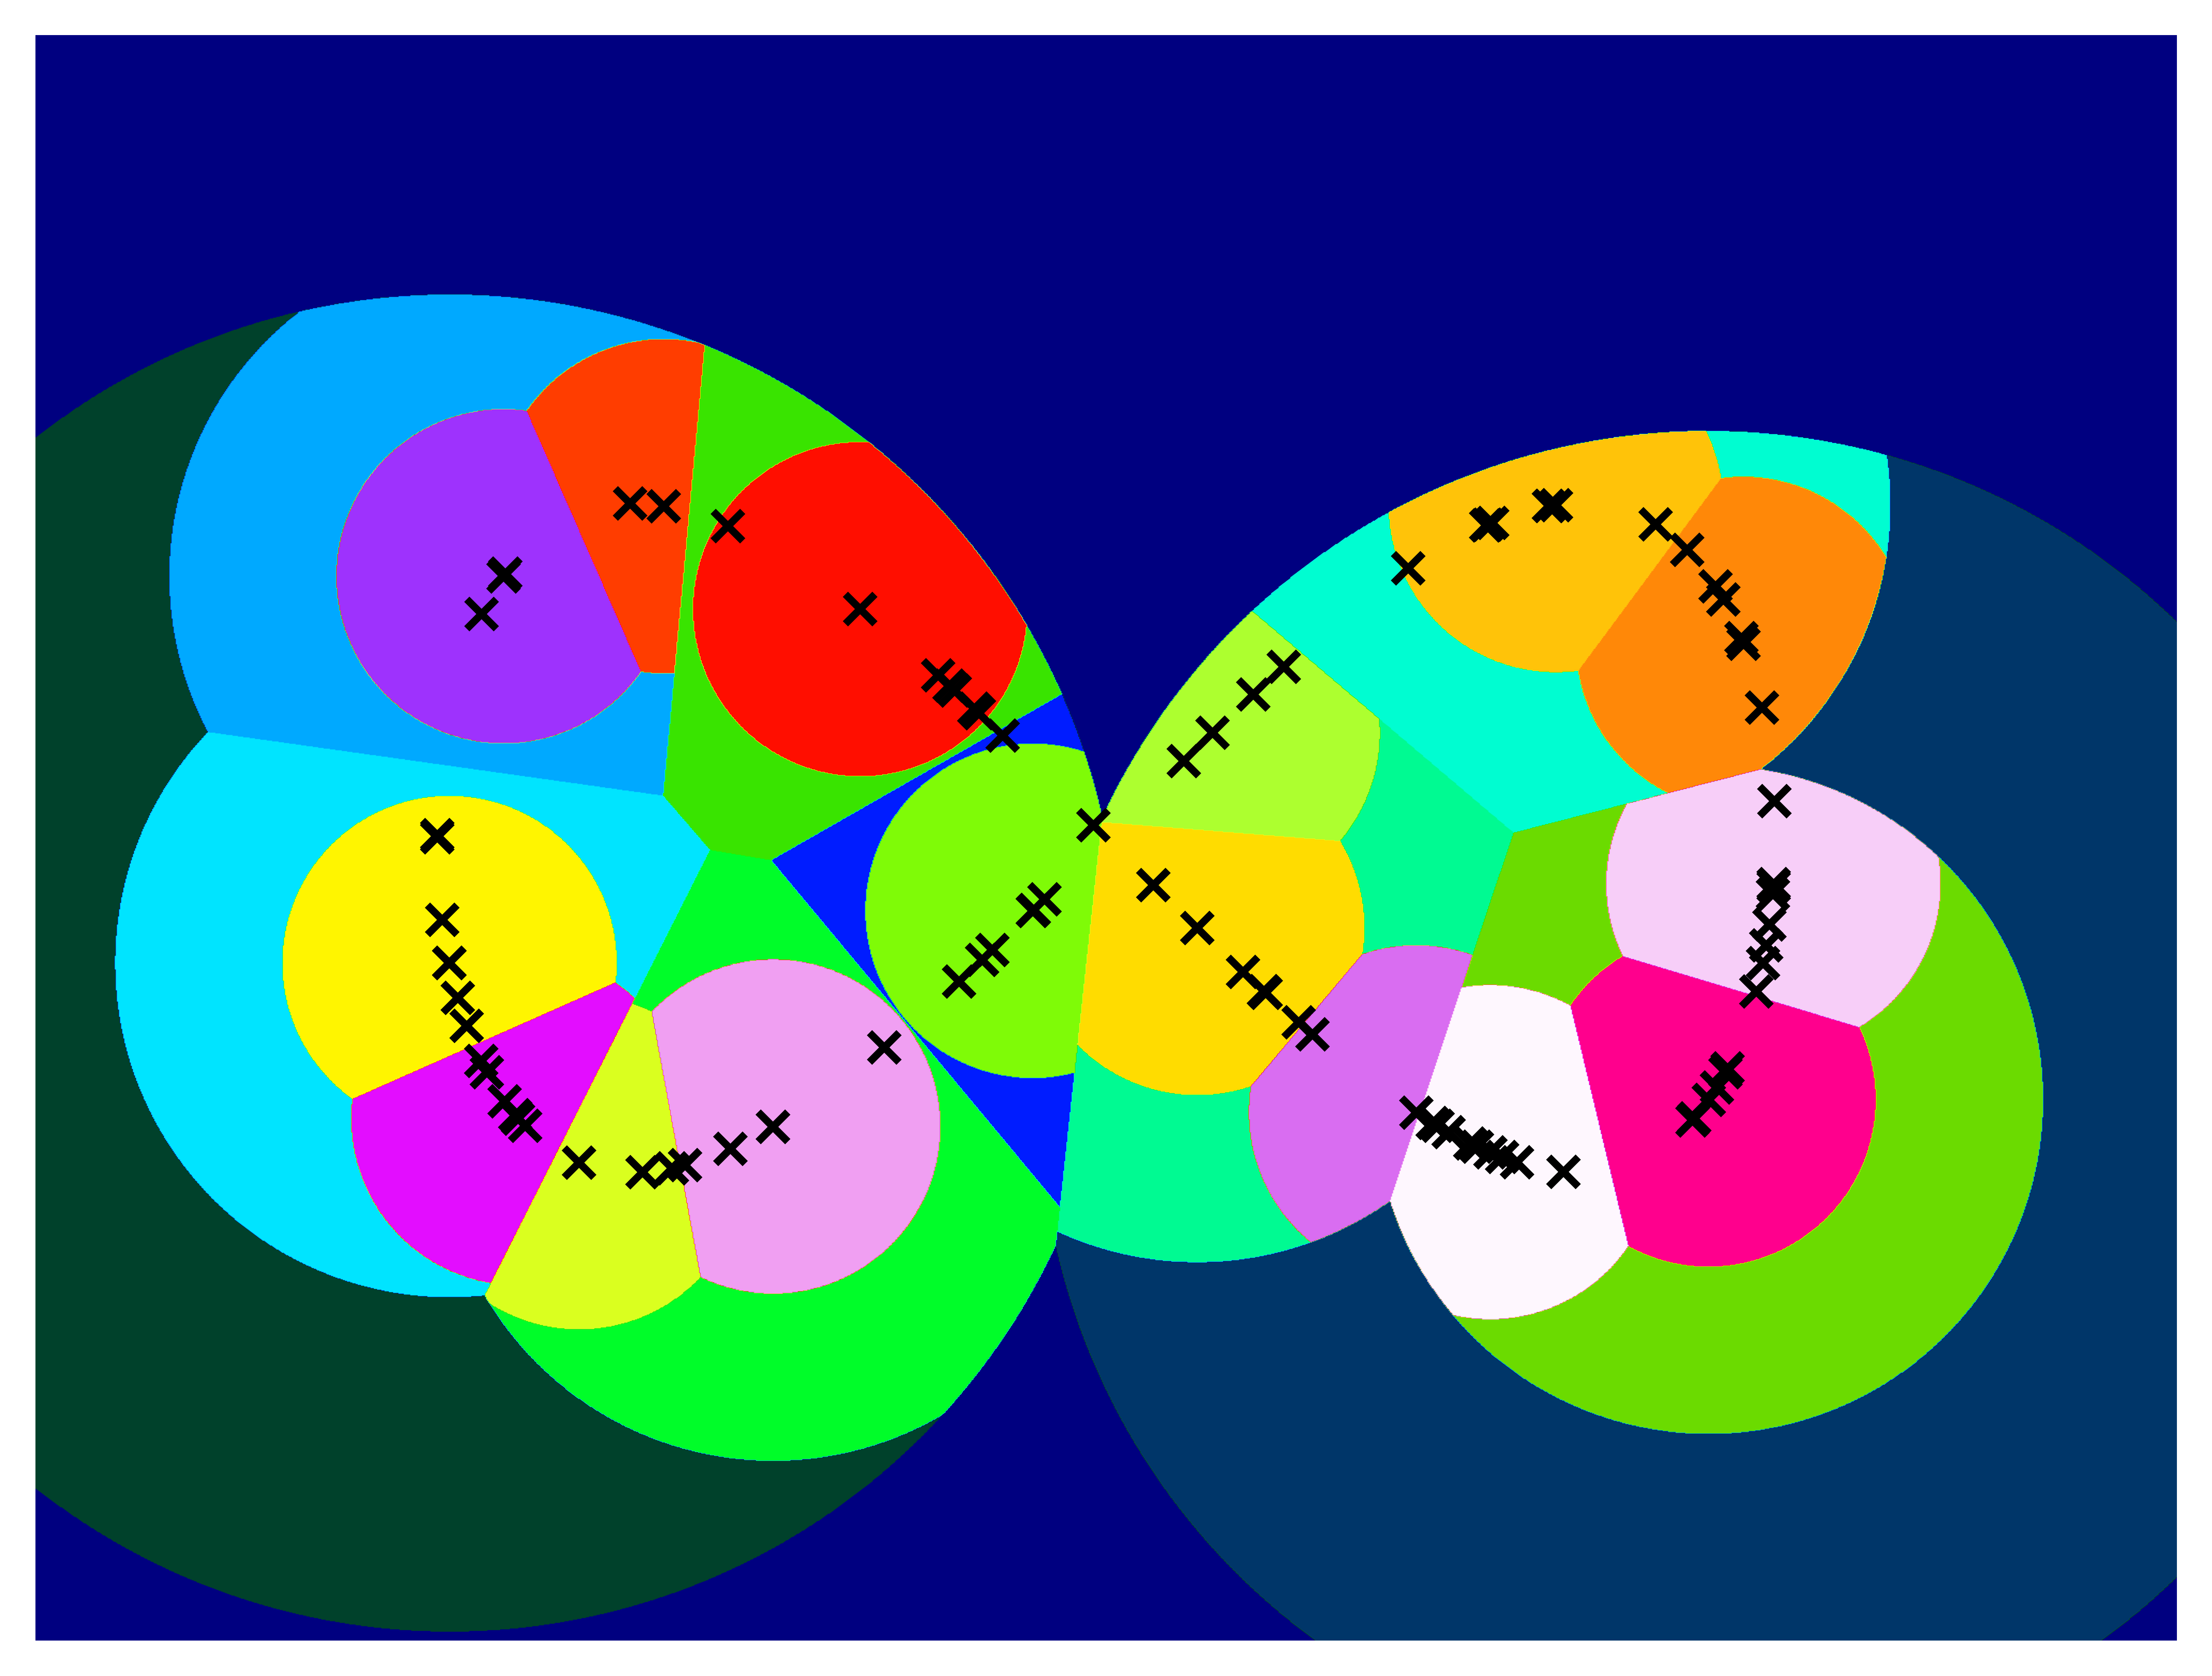
\includegraphics[scale=0.6]{partition_3.png}
\end{center}
\end{frame}

\begin{frame}
\frametitle{How A Covertree Partitions Space, Level -3}
\begin{center}
    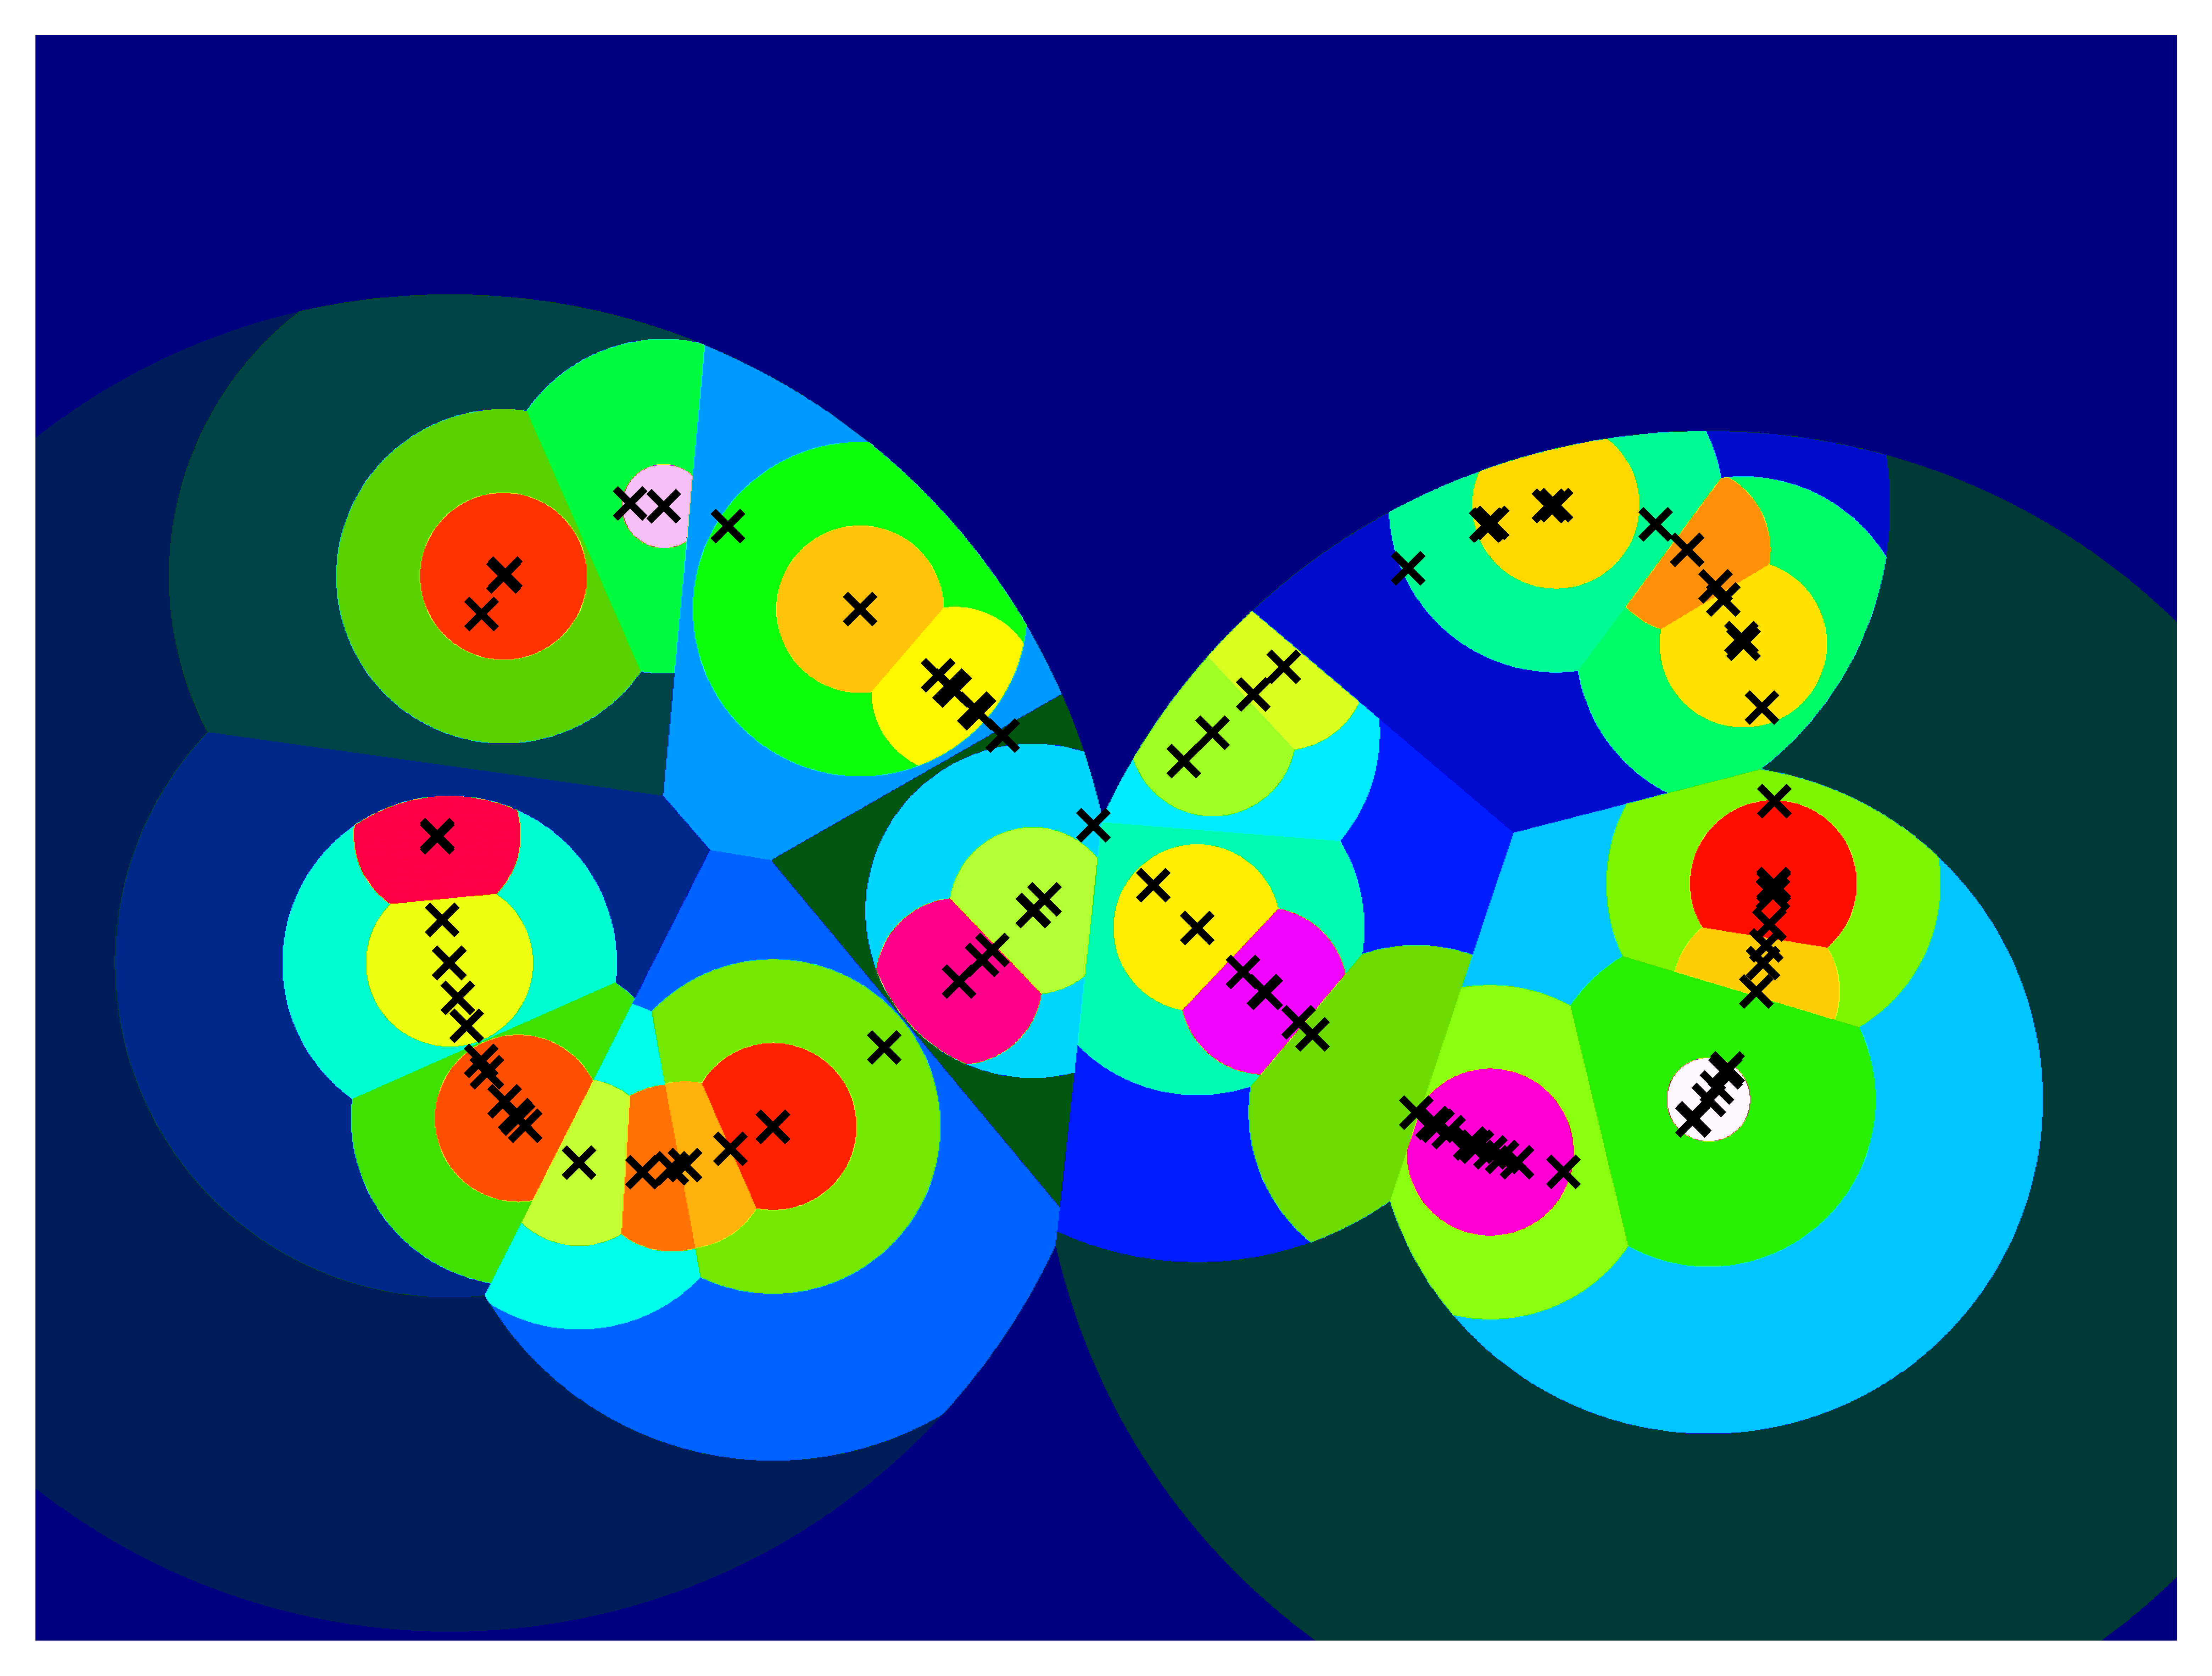
\includegraphics[scale=0.6]{partition_4.png}
\end{center}
\end{frame}

\begin{frame}
    \frametitle{A simple approximation of the true distribution}
    \begin{itemize}
        \item Each node covers $N$ elements of the tree.
        \item The node's children cover $(N_1, N_2, \dots N_k)$
        \item Therefore the probability of a point associated to the parent node, is associated to the $i$th child node is $\frac{N_i}{N}$
    \end{itemize}
\end{frame}

\begin{frame}
\frametitle{Approximating the Probability Distribution From a Covertree}
\begin{center}
    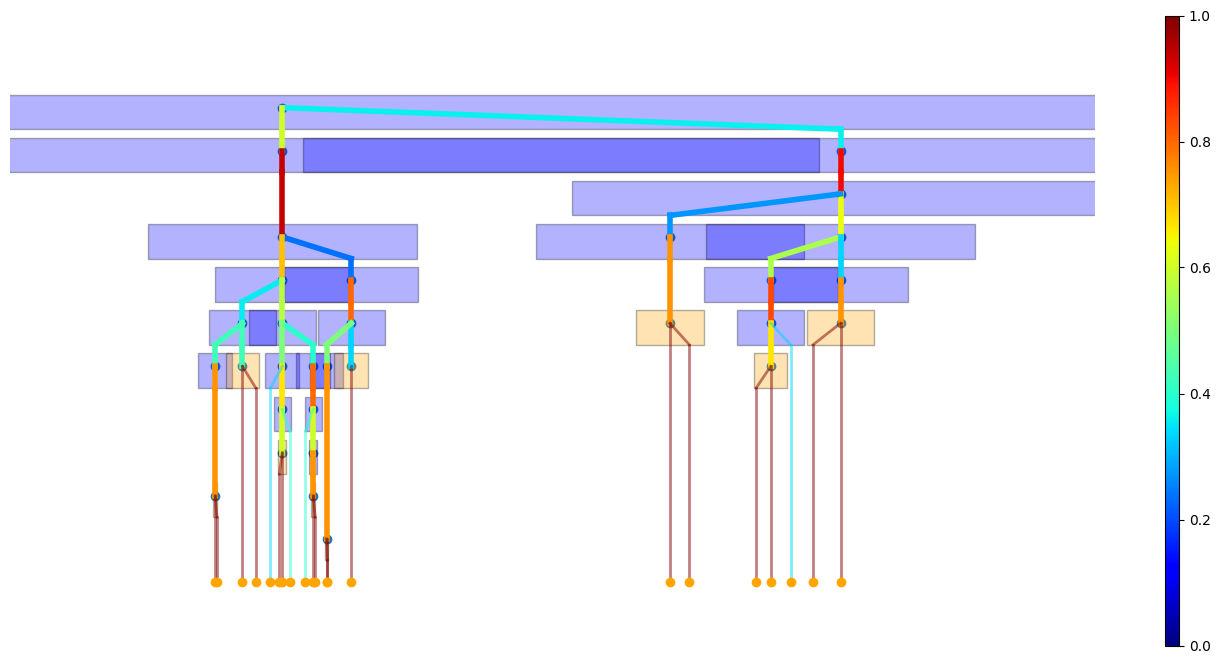
\includegraphics[scale=0.35]{1d_vis_post_prob_0.png}
\end{center}
\end{frame}

\begin{frame}
\frametitle{Oops, The Estimate was Wrong}
\begin{center}
    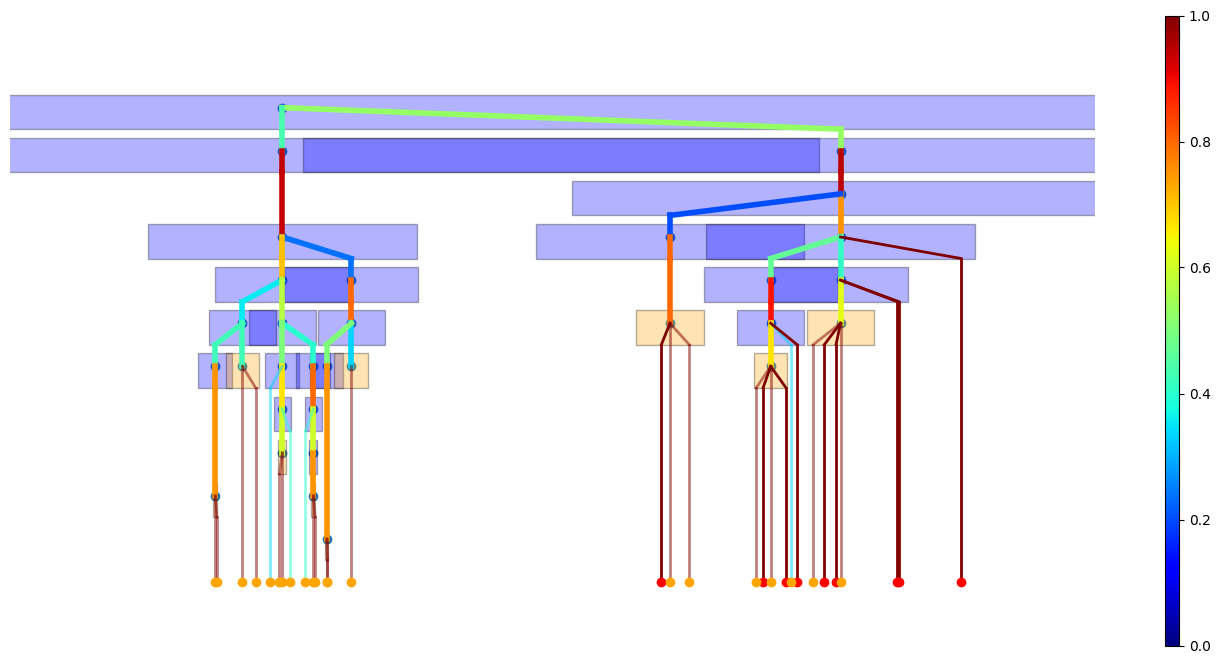
\includegraphics[scale=0.35]{1d_vis_post_prob_9.png}
\end{center}
\end{frame}

\section{Bayesian Background}
\begin{frame}
    \frametitle{Let's be Bayesian about this}
    \begin{itemize}
        \item We know a lot about the root of the tree, lots of observations.
        \item We know little about the leaves of the tree, few observations.
        \item Therefore, model the distribution of distributions, using a Dirichlet distribution.
    \end{itemize}
\end{frame}

\begin{frame}
    \frametitle{A Node's Dirichlet Distribution}
    For node covering $N_0$, with children covering $\alpha = (N_1, \dots, N_k)$, we associate a Dirichlet Distribution
    $\text{Dir}(\alpha)$. The probability density function for this is:
    $$f(x_1, \dots, x_k ; N_1, \dots, N_k) = \frac{\prod_{i=1}^k \Gamma(N_i)}{\Gamma(N_0)} \prod x_i^{N_i - 1}$$
    
    Can also do this with all nodes for the "overall distribution"
\end{frame}

\begin{frame}
    \frametitle{A Dirichlet Visualization \footnote{Source: Wikipedia}}
    \begin{center}
        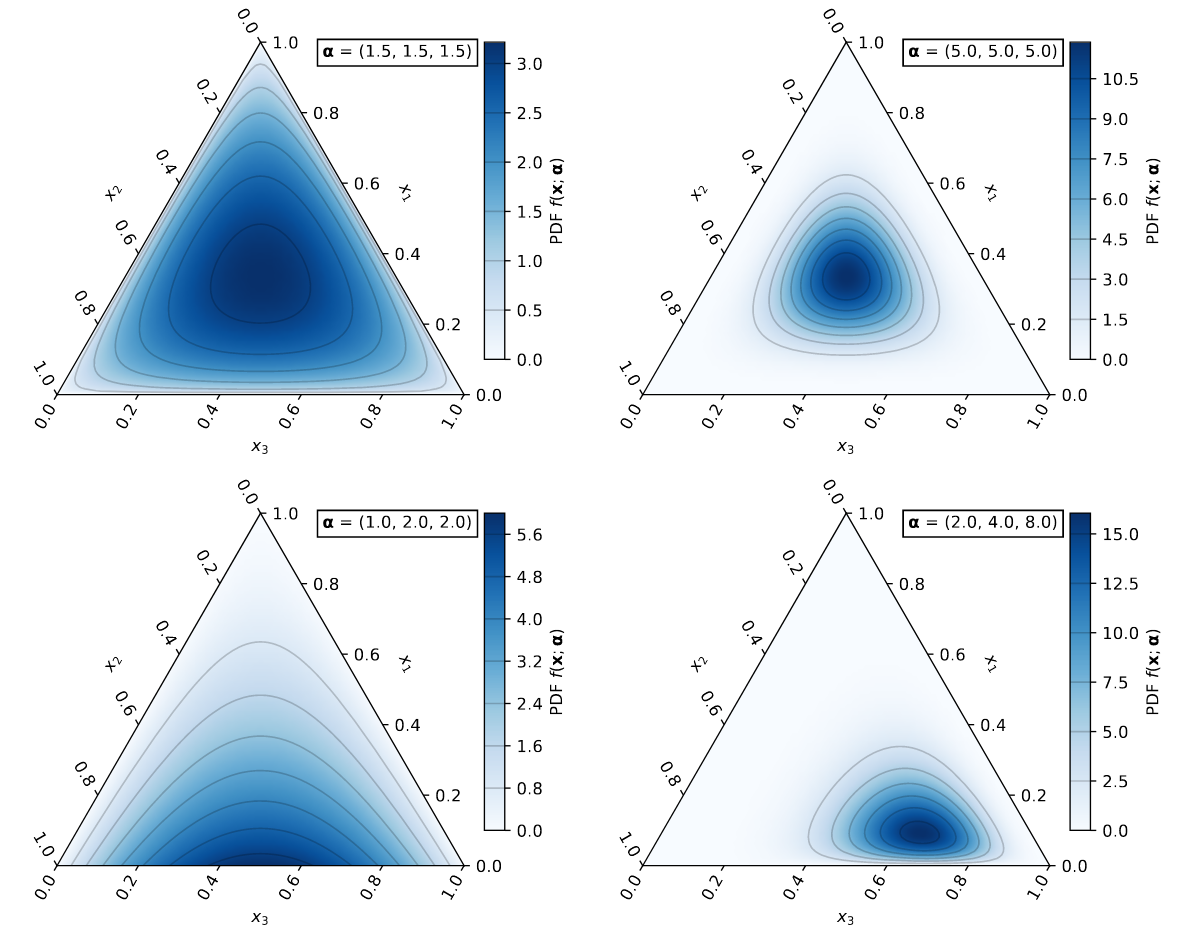
\includegraphics[scale=0.22]{wiki_dirichlet.png}
        
    \end{center}

\end{frame}

\begin{frame}
    \frametitle{Prior VS Posterior}
    The \emph{prior} associated to a node is $\text{Dir}((1, \dots, 1))$. The training posterior is 
    $$P_A = \text{Dir}((N_1 + 1, \dots, N_k + 1)).$$ If there are $O_i$ points in the test set whose paths pass 
    through the $i$th child, then the test-posterior is: $$Q_A = \text{Dir}((N_1 + O_1 + 1, \dots, N_k + O_k + 1)).$$
\end{frame}

\begin{frame}
    \frametitle{Drift Metrics: Kullback–Leibler divergence \footnote{Source: https://bariskurt.com/kullback-leibler-divergence-between-two-dirichlet-and-beta-distributions/}}
    \begin{multline}
        \text{KL}(Q_A||P_A) = \log \Gamma(N_0) - \log \Gamma(N_0 + O_0) + \\ \sum_{i=1}^k \lbrace \Gamma(N_i + O_i) - \Gamma(N_i) + O_i (\psi(N_i) - \psi(N_0)) \rbrace
    \end{multline}
\end{frame}

\begin{frame}
    \frametitle{Marginal Log Likelihood of Test, Given Observations}
    Model the distributions of multinomial distributions with $O$ samples instead of categorical, then calculate the ln of the marginal distribution:
    \begin{multline}
        \text{MLL}(O|N) = \log \Gamma(N_0) + \log \Gamma(O_0 + 1) - \log \Gamma(N_0 + O_0) + \\ \sum_{i=1}^k \lbrace \Gamma(N_i + O_i) - \Gamma(N_i) - \Gamma(O_i + 1) \rbrace
    \end{multline}
\end{frame}

\begin{frame}
    \frametitle{Visualization Of KL Div VS MLL}
    \begin{center}
        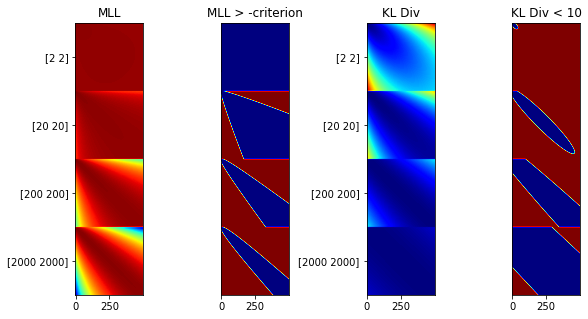
\includegraphics[scale=0.5]{goodness_of_fit.png}
    \end{center}
\end{frame}

\section{Method}
\begin{frame}
    \frametitle{Let's build some intuition}
    \begin{enumerate}
        \item Our training set will be 10000 points from a 2D daussian.
        \item Or test sets will be 1000, and 10000 points sampled from the same gaussian.
        \item We'll sample the attack point from the same gaussian.
        \item We'll replace 0\%, 1\% and 10\% of the test set with the attack point, these are the attack rates. 
    \end{enumerate} 
\end{frame}

\begin{frame}
    \frametitle{Visualization Of Gaussian Toy}
    \begin{center}
        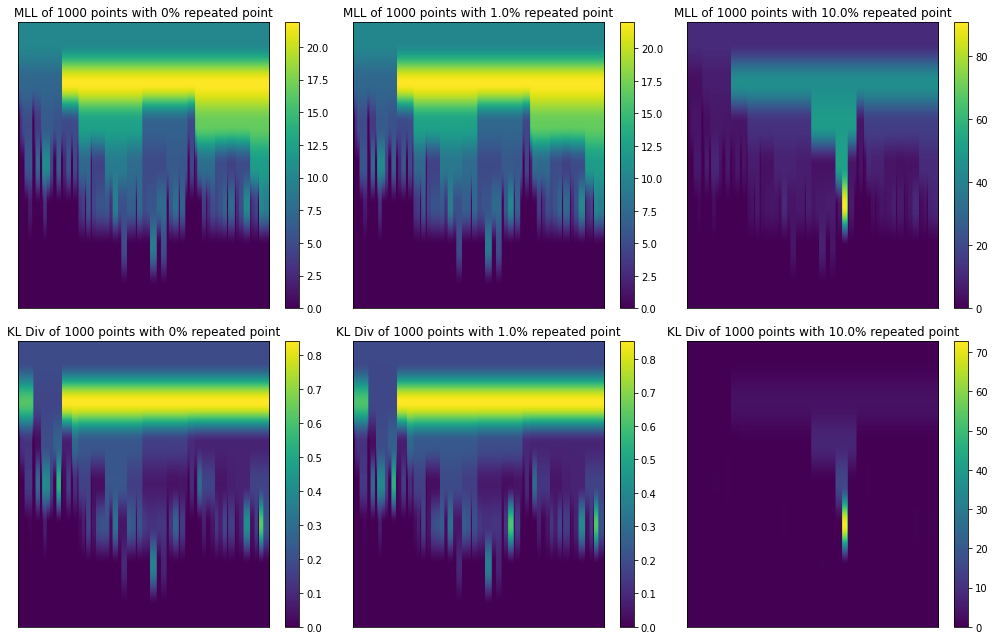
\includegraphics[scale=0.3]{tree_val_plot_1000.png}
    \end{center}
\end{frame}

\begin{frame}
    \frametitle{Visualization Of Gaussian Toy}
    \begin{center}
        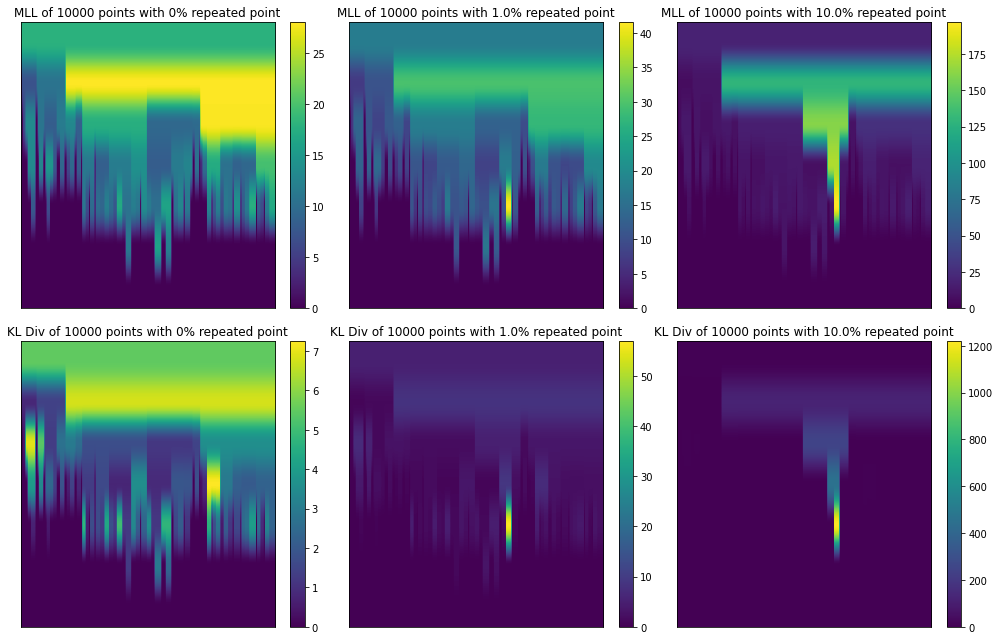
\includegraphics[scale=0.3]{tree_val_plot_10000.png}
    \end{center}
\end{frame}

\begin{frame}
    \frametitle{How to do Classification}
    Take a baseline, $B$, run some sequences through the covertree's tracker and calculate the per-node maximum, and standard deviation.
    
    $$ \widehat{\text{KL}}_B(Q_a|| P_a) = \text{KL}(Q_a|| P_a) - \max_B \text{KL}(Q_a|| P_a) - S_{\text{KL}} \sigma_\text{KL} - C_{\text{KL}}$$
    $$ \widehat{\text{MLL}}_B(O|| N) = \text{MLL}(O|| N)  - \max_{b \in B} \text{MLL}(O_b|| N_b) - S_{\text{MLL}} \sigma_\text{MLL} - C_{\text{MLL}}$$
    \begin{center}
        
\includegraphics[scale=0.3]{nuke_it_from_orbit.png}
    \end{center}
\end{frame}

\begin{frame}
    \frametitle{Visualization Of Gaussian Toy}
    \begin{center}
        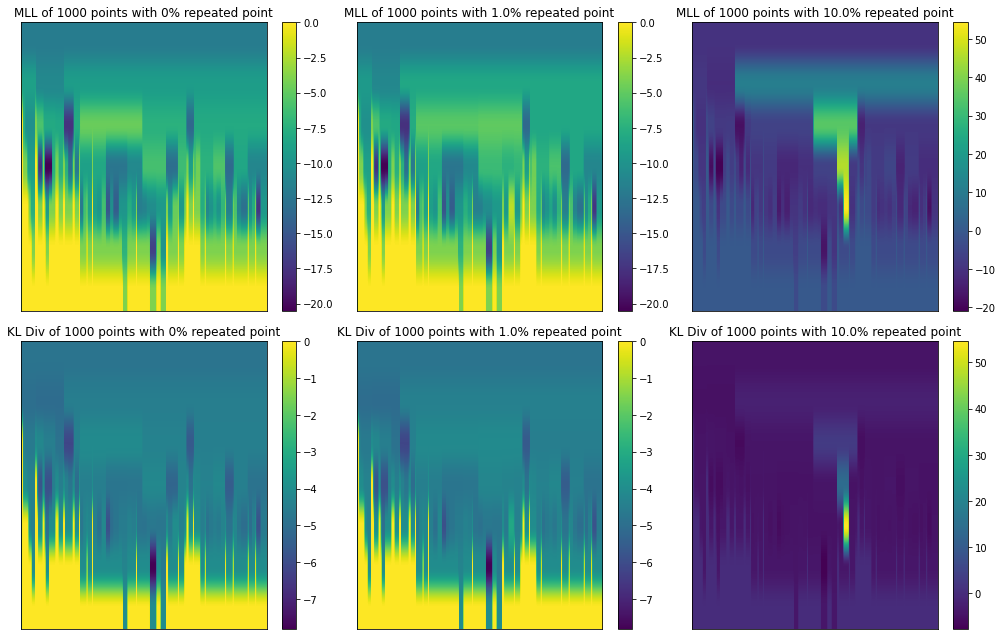
\includegraphics[scale=0.3]{tree_val_plot_1000_minus_baseline.png}
    \end{center}
\end{frame}

\begin{frame}
    \frametitle{Visualization Of Gaussian Toy}
    \begin{center}
        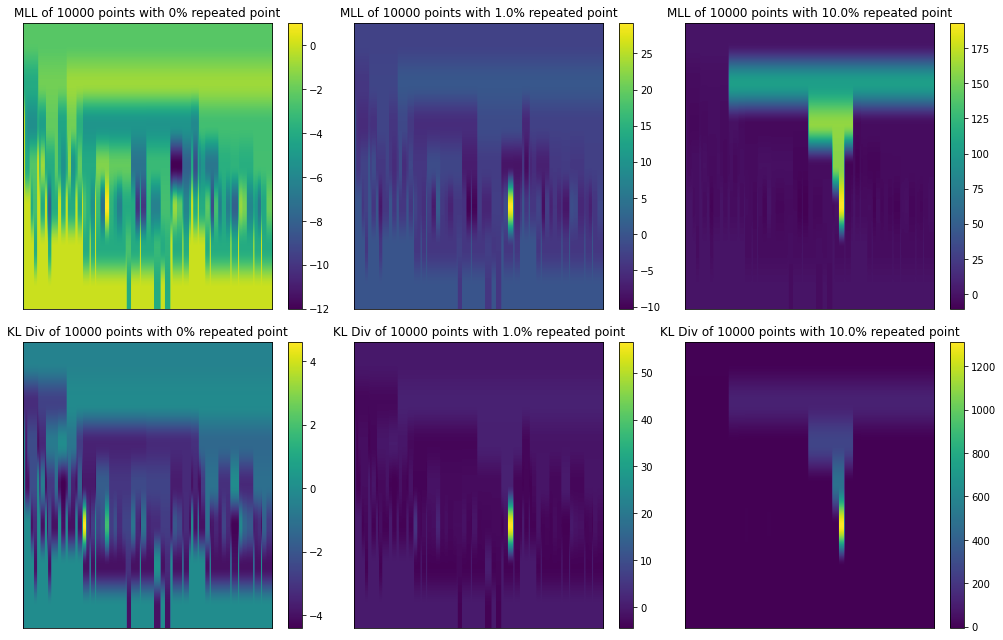
\includegraphics[scale=0.3]{tree_val_plot_10000_minus_baseline.png}
    \end{center}
\end{frame}

\begin{frame}
    \frametitle{Definition of Detection}
    A "detection" is performed in 2 passes, the first is the address of the node with the maximal positive $\widehat{\text{KL}}_B(Q_a|| P_a)$.
    
    If $\widehat{\text{KL}}_B(Q_a|| P_a)$ is everywhere non-positive, the address of the node with maximal positive $\widehat{\text{MLL}}_B(O|| N)$.
    
    If both terms are non-positive for all nodes, nothing is detected. 
\end{frame}

\section{Results}

\begin{frame}
    \frametitle{Overall KL Divergence of SOREL's test set}
    \begin{tabular}{| r | c c | c c | c c |}
        \hline
         & \multicolumn{6}{|c|}{Window size} \\
        \hline
         & \multicolumn{2}{|c|}{1000} & \multicolumn{2}{|c|}{10000} & \multicolumn{2}{|c|}{100000} \\
        \hline
        Attack Rate & $\mu$ & $\sigma$ & $\mu$ & $\sigma$ & $\mu$ & $\sigma$ \\
        \hline
        0.0 & 0.0 & 1.0 & 0.0 & 1.0 & 0.0 & 1.0 \\
        \hline
        0.0001 & 8e-5 & 1.0 & 3e-5 & 1.0 & 2e-5 & 0.999 \\
        \hline
        0.001 & 0.0001 & 0.99 & 0.0003 & 1.0 & 0.0004 & 1.0 \\
        \hline
        0.01 & 0.007 & 1.03 & 0.009 & 1.06 & 0.014 & 1.095 \\
        \hline
        0.10 & 0.293 & 4.025 & 0.299 & 4.167 & 0.329 & 4.122 \\
        \hline
        1.00 & 10.172 & 55.40 & 7.379 & 41.376 & 5.987 & 36.260 \\
        \hline
    \end{tabular}
\end{frame}

\begin{frame}
    \frametitle{Overall Marginal Log Likelihood of SOREL's test set}
    \begin{tabular}{| r | c c | c c | c c |}
        \hline
         & \multicolumn{6}{|c|}{Window size} \\
        \hline
         & \multicolumn{2}{|c|}{1000} & \multicolumn{2}{|c|}{10000} & \multicolumn{2}{|c|}{100000} \\
        \hline
        Attack Rate & $\mu$ & $\sigma$ & $\mu$ & $\sigma$ & $\mu$ & $\sigma$ \\
        \hline
        0.0 & 0.0 & 1.0 & 0.0 & 1.0 & 0.0 & 1.0 \\
        \hline
        0.0001 & -0.0006 & 1.0 & -0.0014 & 1.0 & -0.0053 & 1.00 \\
        \hline
        0.001 & -0.004 & 0.99 & -0.04 & 1.0 & -0.16 & 1.00 \\
        \hline
        0.01 & -0.18 & 1.03 & -0.92 & 1.08 & -2.70 & 1.095 \\
        \hline
        0.10 & -3.78 & 1.66 & -13.45 & 1.75 & -32.26 & 1.38 \\
        \hline
        1.00 & -53.91 & 4.382 & -160.87 & 2.78 & -407.52 & 1.456 \\
        \hline
    \end{tabular}
\end{frame}

\begin{frame}
    \frametitle{SOREL Baseline Adjustment}
    Took a baseline, with a validation set. Did leave one out cross validation and adjusted the 4 hyperparameters until the following saw next to no FPS. There's an extra term $\omega$ called the \emph{margin of safety}. I used $1.5$.
    $$ \widehat{\text{KL}}_B(Q_a|| P_a) = \omega \text{KL}(Q_a|| P_a) - \max_B \text{KL}(Q_a|| P_a) - S_{\text{KL}} \sigma_\text{KL} - C_{\text{KL}}$$
    $$ \widehat{\text{MLL}}_B(O|| N) = \omega \text{MLL}(O|| N)  - \max_{b \in B} \text{MLL}(O_b|| N_b) - S_{\text{MLL}} \sigma_\text{MLL} - C_{\text{MLL}}$$
\end{frame}

\begin{frame}
    \frametitle{Visualization Of SOREL Baseline Adjustment for 1000}
    \begin{center}
        \includegraphics[scale=0.4]{1000_violators.png}
    \end{center}
\end{frame}

\begin{frame}
    \frametitle{Visualization Of SOREL Baseline Adjustment for 10000}
    \begin{center}
        \includegraphics[scale=0.4]{10000_violators.png}
    \end{center}
\end{frame}

\begin{frame}
    \frametitle{Visualization Of SOREL Baseline Adjustment for 100000}
    \begin{center}
        \includegraphics[scale=0.4]{100000_violators.png}
    \end{center}
\end{frame}

\begin{frame}
    \frametitle{Safe Baseline Hyperparameter Results}
    With a safety margin of 2.
    \begin{center}
        \begin{tabular}{| r | c c | c c |}
        \hline
        Window Size & $S_{KL}$ & $C_{KL}$ & $S_{ML}$ & $C_{ML}$ \\
        \hline 
        1000 & 10 & 12 & 1.3 & 80 \\
        \hline 
        10000 & 20 & 6.5 & 1.4 & 100 \\
        \hline 
        100000 & 15 & 80 & 1.9 & 100 \\
        \hline 
    \end{tabular}
    \end{center}
\end{frame}

\begin{frame}
    \frametitle{Safe Test Set Results}
    \begin{center}
        \begin{tabular}{| r | r | c c c c c c |}
        \hline
         & & \multicolumn{6}{|c|}{Attack Rates} \\
        \hline
        \multicolumn{2}{|c|}{Window Size} & 0\% & 0.01\% & 0.1\% & 1\% & 10\% & 100\% \\
        \hline
        \multirow{3}{*}{1000} & TPR & 0 & 0 & 0 & 0.7 & 88 & 100 \\
                              & FPR & 0 & 0 & 0 &   0 &  0 & 0 \\
                              & MDR &   - &   - &   - &  96 & 87 &  93 \\
        \hline
        \multirow{3}{*}{10000} & TPR & 0 & 0 & 0.7 & 63.7 & 99.95 & 100 \\
                               & FPR & 0 & 0 &   0 &    0 &     0 & 0 \\
                               & MDR &   - &   - &  96 &   93 &    93 & 91 \\
        \hline
        \multirow{3}{*}{100000} & TPR &   0 & 0.1 & 22.7 & 98.4 & 100 & 100 \\
                                & FPR & 0.4 & 0.3 &    0 &    0 &   0 & 0 \\
                                & MDR &     - &  85 &   94 &   93 &  92 & 88 \\
        \hline
    \end{tabular}
    \end{center}
    Mean Depth Rate - Detection depth of attack over the final depth. 
    
    All values in percentages. Averaged over 1972 runs with 48 different trees.
\end{frame}

\begin{frame}
    \frametitle{Not So Safe Baseline Hyperparameter Results}
    With a safety margin of 1.3.
    \begin{center}
        \begin{tabular}{| r | c c | c c |}
        \hline
        Window Size & $S_{KL}$ & $C_{KL}$ & $S_{ML}$ & $C_{ML}$ \\
        \hline 
        1000 & 8 & 7 & 1.3 & 20 \\
        \hline 
        10000 & 10 & 6.5 & 1.3 & 20 \\
        \hline 
        100000 & 10 & 40 & 1.7 & 50 \\
        \hline 
    \end{tabular}
    \end{center}
\end{frame}

\begin{frame}
    \frametitle{Not So Safe Test Set Attack Results for SOREL}
    \begin{center}
        \begin{tabular}{| r | r | c c c c c c |}
        \hline
         & & \multicolumn{6}{|c|}{Attack Rates} \\
        \hline
        \multicolumn{2}{|c|}{Window Size} & 0\% & 0.01\% & 0.1\% & 1\% & 10\% & 100\% \\
        \hline
        \multirow{3}{*}{1000} & TPR & 0 & 0 & 0 & 16.6 & 96 & 100 \\
                              & FPR & 0 & 0 & 0 &    0 &  0 &   0 \\
                              & MDR &   - &   - &   - &   94 & 89 &  93 \\
        \hline
        \multirow{3}{*}{10000} & TPR & 0 & 0 &  5 &  81 & 99.95 & 100 \\
                               & FPR & 0 & 0 &  0 &   0 &     0 &   0 \\
                               & MDR &   - &   - & 94 &  91 &    93 &  91 \\
        \hline
        \multirow{3}{*}{100000} & TPR &   0 & 0.2 & 44.5 & 98.4 & 100 & 100 \\
                                & FPR & 0.1 & 0.9 &  0.6 &    0 &   0 & 0 \\
                                & MDR &     - &  84 &   94 &   94 &  92 & 88 \\
        \hline
    \end{tabular}
    \end{center}
    Mean Depth Rate - Detection depth of attack over the final depth. 
    
    All values in percentages. Averaged over 1972 runs with 48 different trees.
\end{frame}

\end{document}